\documentclass[12pt,a4paper]{article}

% ── Typography ──
\usepackage[T1]{fontenc}
\usepackage{mathpazo}           % Palatino for body + math
\usepackage{inconsolata}        % monospace
\linespread{1.15}               % comfortable reading

% ── Layout ──
\usepackage[margin=1in]{geometry}
\geometry{headheight=15pt}
\usepackage{fancyhdr}
\pagestyle{fancy}
\fancyhf{}
\fancyhead[L]{\small\itshape Foundation Model for Wireless Communication}
\fancyhead[R]{\small\itshape UGP Report}
\fancyfoot[C]{\thepage}
\setlength{\parindent}{1.2em}
\setlength{\parskip}{0.4em}

% ── Maths & Symbols ──
\usepackage{amsmath,amssymb,amsfonts,bm}
\usepackage{textcomp}

% ── Graphics & Figures ──
\usepackage{graphicx}
\usepackage[font=small,labelfont=bf,skip=6pt]{caption}
\usepackage{subcaption}
\usepackage{float}
\usepackage{tikz}
\usetikzlibrary{shapes.geometric, arrows.meta, positioning, fit, calc, backgrounds}
\usepackage{microtype}          % Better hyphenation and spacing
\usepackage{url}                % Handle long URLs

% ── Tables ──
\usepackage{booktabs}
\usepackage{array}
\usepackage{multirow}

% ── Lists ──
\usepackage{enumitem}
\setlist{nosep, leftmargin=1.5em}

% ── Misc ──
\usepackage{xcolor}
\usepackage{hyperref}
\hypersetup{
  colorlinks=true,
  linkcolor=blue!50!black,
  citecolor=green!40!black,
  urlcolor=blue!60!black
}

% ── Custom colours ──
\definecolor{iitkorange}{RGB}{204,85,0}
\definecolor{blockblue}{RGB}{230,240,250}
\definecolor{blockorange}{RGB}{255,240,225}

% ════════════════════════════════════════════════════════════════
\begin{document}

% ── TITLE PAGE ─────────────────────────────────────────────────
\begin{titlepage}
\centering

\vspace*{0.4cm}

\includegraphics[width=3.2cm]{iitk_logo.png}

\vspace{0.4cm}
{\Large\bfseries Indian Institute of Technology Kanpur}\\[4pt]
{\large Department of Electrical Engineering}

\vspace{1.5cm}

\rule{\textwidth}{1.6pt}\\[0.5cm]
{\LARGE\bfseries Foundation Model for\\[8pt] Wireless Communication}\\[0.5cm]
\rule{\textwidth}{1.6pt}

\vspace{1.2cm}
{\Large\bfseries Undergraduate Project (UGP) Report}

\vspace{1.5cm}

\begin{minipage}[t]{\textwidth}\centering
  {\large\bfseries Supervisor}\\[8pt]
  {\large Prof.\ Rohit Budhiraja}\\[4pt]
  Department of Electrical Engineering\\
  IIT Kanpur
\end{minipage}

\vspace{1.2cm}

\begin{minipage}[t]{0.44\textwidth}\centering
  {\large\bfseries Student}\\[8pt]
  {\large Ronit Kumar}\\[4pt]
  Department of Electrical Engineering\\
  IIT Kanpur
\end{minipage}
\hfill
\begin{minipage}[t]{0.44\textwidth}\centering
  {\large\bfseries Student}\\[8pt]
  {\large Udbhav Agarwal}\\[4pt]
  Department of Electrical Engineering\\
  IIT Kanpur
\end{minipage}

\vfill
{\large May 2026}
\end{titlepage}

% ── TABLE OF CONTENTS ──────────────────────────────────────────
\pagenumbering{roman}
\tableofcontents
\newpage
\pagenumbering{arabic}

% ══════════════════════════════════════════════════════════════
%  ABSTRACT
% ══════════════════════════════════════════════════════════════
\begin{abstract}
\noindent
The Large Wireless Model (LWM)~\cite{lwm} is a transformer-based foundation model that is pre-trained in a self-supervised fashion on large-scale wireless channel data using a masked channel modelling (MCM) objective.  Although LWM produces rich, context-aware channel embeddings that benefit a variety of downstream tasks, the original system leaves two important dimensions largely unexplored: the design of the downstream prediction head and the computational efficiency of the backbone itself.

This report documents four phases of work carried out during the undergraduate project.
In \textbf{Phase~1}, we replace the baseline Residual CNN (ResCNN) downstream head with a Squeeze-and-Excitation CNN (SECNN), achieving consistent improvements across all training-data regimes.
In \textbf{Phase~2}, we integrate three attention mechanisms  Coordinate Attention, Axial Attention, and Physics-guided attention  directly into the LWM~1.0 encoder and benchmark them on the beam prediction task; Coordinate Attention emerges as the strongest variant.
In \textbf{Phase~3}, we port Coordinate Attention to the newer LWM~1.1 backbone and compare its performance against LWM~1.0, observing that while LWM~1.1 under-performs LWM~1.0 in the base configuration, the addition of Coordinate Attention narrows the gap noticeably.
In \textbf{Phase~4}, we explore the Mask-Aware Transformer (MAT)~\cite{mat} as a lighter-weight backbone, developing four architectural variants; the best variant (MAT-Pseudo) matches or exceeds the base LWM~1.0 at roughly one-half the FLOPs and one-third the parameters.

The present report covers Phase~1 in full detail; subsequent phases will be documented incrementally.
\end{abstract}

% ══════════════════════════════════════════════════════════════
%  1. INTRODUCTION
% ══════════════════════════════════════════════════════════════
\newpage
\section{Introduction}\label{sec:intro}

Current and future wireless communication and sensing systems promise substantial performance gains by relying on massive antenna arrays, high-frequency bands (mmWave and sub-terahertz), and dense network deployments. However, realizing this potential requires overcoming critical challenges in high-dimensional signal processing, massive wireless overhead, and complex network optimization. While deep learning offers powerful data-driven solutions to these problems, traditional models often struggle to generalize across diverse, dynamic wireless environments and heavily depend on large labeled datasets which are typically scarce and expensive to collect.

To address these fundamental limitations, the paradigm of foundation models has recently been adapted to wireless communications. The \textbf{Large Wireless Model (LWM)}~\cite{lwm} represents a pioneering step in this direction: it is a transformer-based foundation model pre-trained in a self-supervised manner on a massive corpus of synthetic wireless channels. By employing a \emph{Masked Channel Modelling} (MCM) objective similar to techniques that have revolutionized natural language processing (BERT) and computer vision (ViT), LWM learns to extract rich, universal, and context-aware channel embeddings. These embeddings act as a powerful universal feature extractor that can be transferred to various downstream tasks, significantly improving performance and reducing the reliance on extensive labeled task-specific data.

While LWM successfully demonstrates the viability of foundation models in wireless systems, maximizing its efficiency and downstream capability remains an active area of research. In this project, we focus on enhancing the LWM framework across two main dimensions: feature representation quality and computational efficiency. To rigorously benchmark the impact of our architectural improvements, we utilize \emph{beam prediction}, a critical task for mmWave systems involving the rapid identification of optimal directional beams, as our primary downstream evaluation task. 

Despite LWM's strong baseline performance, several avenues remain open for further improvement:

\paragraph{Downstream head design.}
The default downstream classifier shipped with LWM is a simple 1-D Residual CNN (ResCNN). This architecture treats all feature channels uniformly and applies aggressive spatial down-sampling. A more expressive downstream head that adaptively weighs important features could extract greater value from LWM's fixed embeddings, particularly in low-data regimes where extracting maximum information is critical.

\paragraph{Backbone attention mechanisms.}
The vanilla multi-head self-attention in LWM effectively captures global channel dependencies but lacks explicit inductive biases for coordinate-level or physical structure. Integrating specialized attention modules such as Coordinate Attention or Physics-guided attention directly into the backbone could yield more informative, structurally-aware embeddings.

\paragraph{Computational efficiency.}
LWM's 12-layer transformer encoder is computationally heavy, posing challenges for real-time inference on resource-constrained edge devices. Developing lighter backbone architectures that maintain or exceed prediction quality at a fraction of the computational cost (FLOPs) is essential for practical deployment.

\subsection{Objectives and Scope}

Motivated by the above considerations, this project pursues two complementary goals: \emph{(i)}~improving prediction quality by upgrading both the downstream head and the backbone attention, and \emph{(ii)}~reducing computational cost by exploring alternative backbone architectures.  The work is organised into four phases:

\begin{enumerate}
  \item \textbf{Phase 1: Downstream head improvement.}  We design a Squeeze-and-Excitation CNN (SECNN) that incorporates channel attention, preserves spatial resolution, and employs a simpler classifier head.  We benchmark it against the original ResCNN on the beam prediction task using both CLS and channel embeddings at six training-data split ratios.

  \item \textbf{Phase 2: Attention integration in LWM\,1.0.}  We integrate Coordinate Attention, Axial Attention, and Physics-guided attention into the LWM encoder and evaluate their impact on beam prediction.  Coordinate Attention is identified as the best-performing variant.

  \item \textbf{Phase 3: Experiments with LWM\,1.1.}  We port Coordinate Attention to the newer LWM\,1.1 backbone and compare performance against LWM\,1.0, analysing the interplay between backbone version and attention augmentation.

  \item \textbf{Phase 4: Mask-Aware Transformer backbone.}  We develop four MAT-based backbone variants and benchmark them on beam prediction.  The MAT-Pseudo variant achieves competitive performance at roughly half the FLOPs and one-third the parameters of LWM\,1.0.
\end{enumerate}

% ══════════════════════════════════════════════════════════════
%  2. BACKGROUND
% ══════════════════════════════════════════════════════════════
\newpage
\section{Background}\label{sec:background}

This section reviews the key building blocks that underpin the experimental work reported in subsequent sections: the LWM architecture, the beam prediction task, and the evaluation methodology.

\subsection{The Large Wireless Model}\label{subsec:lwm}

LWM is a 12-layer transformer encoder whose hyper-parameters are summarised in Table~\ref{tab:lwm_config}.  The input to the model is a wireless channel matrix $\mathbf{H}\in\mathbb{C}^{M\times N}$ with $M=32$ base-station antennas and $N=32$ OFDM sub-carriers.

\begin{table}[h]
\centering
\caption{LWM encoder hyper-parameters.}
\label{tab:lwm_config}
\begin{tabular}{@{}lc@{}}
\toprule
\textbf{Parameter} & \textbf{Value} \\
\midrule
Encoder layers       & 12 \\
Hidden dimension $d_{\text{model}}$   & 64 \\
Attention heads      & 12 \\
Head dimension $d_k = d_v$ & $64/12$ \\
Feed-forward dim $d_{\text{ff}}$ & 256 \\
Patch size $L$       & 16 \\
Number of patches $P$& 128 \\
Sequence length (with \texttt{[CLS]}) & 129 \\
Dropout              & 0.1 \\
\bottomrule
\end{tabular}
\end{table}

\paragraph{Patch generation.}
The channel matrix is first separated into its real and imaginary components, $\mathbf{H}_{\text{real}}=\Re(\mathbf{H})$ and $\mathbf{H}_{\text{imag}}=\Im(\mathbf{H})$, each of which is flattened into a vector of length $MN=1024$.  Concatenating these vectors yields a real-valued representation $\mathbf{h}\in\mathbb{R}^{2MN}$ of length 2048.  This vector is then divided into $P=128$ non-overlapping patches of size $L=16$:
\begin{equation}
  \mathbf{p}_i = \mathbf{h}\bigl[(i-1)L+1 \,:\, iL\bigr], \quad i=1,\dots,P.
  \label{eq:patches}
\end{equation}

\paragraph{Embedding and positional encoding.}
Each patch $\mathbf{p}_i$ is linearly projected to the model dimension via a learnable weight matrix $\mathbf{W}_{\text{proj}}\in\mathbb{R}^{d_{\text{model}}\times L}$, and a learnable positional embedding $\mathbf{e}_i$ is added.  A special \texttt{[CLS]} token $\mathbf{p}_0$ is prepended, yielding an input sequence of length 129:
\begin{equation}
  \mathbf{z}_i^{(0)} = \mathbf{W}_{\text{proj}}\,\mathbf{p}_i + \mathbf{e}_i, \quad i=0,1,\dots,P.
  \label{eq:embed}
\end{equation}

\paragraph{Masked channel modelling.}
During self-supervised pre-training, 15\% of patches are randomly selected and replaced with a learnable \texttt{[MASK]} token (with 10\% probability they are instead replaced by a random vector).  The encoder processes the corrupted sequence through 12 transformer layers.  A lightweight decoder head reconstructs the original patch values at the masked positions, and the model is trained to minimise the mean-squared error between predictions and ground truth.

\paragraph{Embedding extraction.}
After pre-training, the encoder weights are frozen and \textbf{two types of embeddings} are extracted for downstream use.  The \emph{CLS embedding} $\mathrm{emb}_{cls}\in\mathbb{R}^{64}$ is the output at the \texttt{[CLS]} position and serves as a global summary of the channel.  The \emph{channel embedding} $\mathrm{emb}_{channel}\in\mathbb{R}^{128\times 64}$, comprising the outputs at all 128 patch positions, preserves fine-grained spatial and spectral structure.

\subsection{Beam Prediction Task}\label{subsec:beam}

The downstream task considered throughout this project is \emph{beam prediction}.  A codebook of $N_b=64$ beams is constructed from a uniform angular grid spanning a 180\textdegree{} field of view.  For each user, the steering vector corresponding to each beam angle $\phi_k$ is applied to the channel, and the beam that maximises the average received power across sub-carriers is selected as the ground-truth label.  Including a ``no-beam'' class, the problem becomes a $(N_b+1)$-class classification task.

\subsection{Evaluation Protocol}\label{subsec:eval}

The dataset comprises 519\,636 channel samples drawn from 19 urban DeepMIMO scenarios.  To study the effect of labelled data availability, we train each downstream model from scratch at six split ratios $r\in\{0.005,\,0.01,\,0.05,\,0.1,\,0.2,\,0.4\}$, where $r$ denotes the fraction used for training.  The remaining $(1-r)$ fraction is divided equally into validation and test sets.  All results are reported as \textbf{weighted F1 scores} on the held-out test set, which appropriately accounts for the inherent class imbalance in beam distributions across diverse urban environments.


% ══════════════════════════════════════════════════════════════
%  3. PHASE 1
% ══════════════════════════════════════════════════════════════
\newpage
\section{Phase 1: Downstream Head Improvement    ResCNN to SECNN}\label{sec:phase1}

The first phase of the project focuses on improving the downstream prediction head while keeping the LWM encoder frozen.  We propose replacing the original Residual CNN (ResCNN) with a Squeeze-and-Excitation CNN (SECNN) that incorporates adaptive channel attention, wider feature maps, and a simplified classifier.

\subsection{Baseline: Residual 1-D CNN (ResCNN)}\label{subsec:rescnn}

The ResCNN architecture provided with LWM follows a standard residual network design adapted for 1-D sequences.  The input embedding (after transposing to channels-first format) passes through a stem convolution with kernel size~7, stride~2, and padding~3, expanding the channel count to~32.  Batch normalisation and ReLU activation follow, and a max-pooling layer with kernel size~3 and stride~2 further halves the spatial dimension.  Three residual stages then process the features with $\{2,3,4\}$ blocks and channel widths $\{32,64,128\}$ respectively.  Each residual block contains two $3\times1$ convolutions with batch normalisation; a $1\times1$ shortcut projection is applied whenever the channel count changes.  After global average pooling, two fully-connected layers (128 and $N_{\text{classes}}$) with an intermediate batch normalisation, ReLU, and dropout of 0.5 produce the final logits.

This design has three notable limitations.  First, all feature channels are treated uniformly  there is no mechanism to emphasise the channels that carry discriminative beam information and suppress those that do not.  Second, the stride-2 stem followed by max-pooling aggressively reduces spatial resolution at the very first layer, discarding fine-grained spectral patterns before the network has had a chance to learn which ones matter.  Third, the high dropout rate of 0.5, while intended to regularise, can lead to under-fitting when training data is already scarce.

\subsection{Squeeze-and-Excitation Mechanism}\label{subsec:se}

The Squeeze-and-Excitation (SE) block addresses the first limitation by adaptively recalibrating channel-wise feature responses.  Given a feature map $\mathbf{U}\in\mathbb{R}^{C\times L}$ with $C$ channels and spatial length $L$, the SE block operates in three stages, illustrated in Figure~\ref{fig:se_block}.

\paragraph{Squeeze.}
A global average pooling operation compresses the spatial dimension into a channel descriptor $\mathbf{z}\in\mathbb{R}^{C}$:
\begin{equation}
  z_c = \frac{1}{L}\sum_{l=1}^{L} u_{c,l}, \quad c=1,\dots,C.
  \label{eq:squeeze}
\end{equation}
This operation aggregates global spatial information into each channel, providing the excitation stage with a receptive field that spans the entire input length.

\paragraph{Excitation.}
A lightweight two-layer fully-connected bottleneck learns non-linear inter-channel dependencies and produces a vector of channel attention weights $\mathbf{s}\in\mathbb{R}^{C}$:
\begin{equation}
  \mathbf{s} = \sigma\!\bigl(\mathbf{W}_2\;\delta(\mathbf{W}_1\,\mathbf{z})\bigr),
  \label{eq:excite}
\end{equation}
where $\mathbf{W}_1\in\mathbb{R}^{(C/r)\times C}$ and $\mathbf{W}_2\in\mathbb{R}^{C\times(C/r)}$ are learnable weight matrices, $r=16$ is the reduction ratio that controls the bottleneck width, $\delta(\cdot)$ denotes the ReLU activation, and $\sigma(\cdot)$ denotes the sigmoid function.

\paragraph{Scale.}
The original feature map is re-weighted channel-wise by the learned attention:
\begin{equation}
  \tilde{u}_{c,l} = s_c \cdot u_{c,l}, \quad \forall\; c,\,l.
  \label{eq:scale}
\end{equation}
Channels deemed important by the excitation network are amplified, while irrelevant or noisy channels are suppressed.

\begin{figure}[H]
\centering
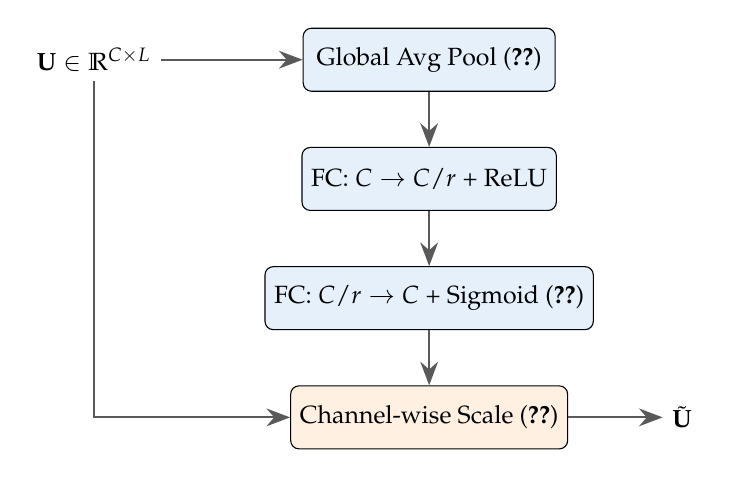
\begin{tikzpicture}[
    block/.style={rectangle, draw, fill=blockblue, minimum width=3.2cm, minimum height=0.8cm, align=center, rounded corners=3pt, font=\small},
    seb/.style={rectangle, draw, fill=blockorange, minimum width=3.2cm, minimum height=0.8cm, align=center, rounded corners=3pt, font=\small},
    arr/.style={-{Stealth[length=3mm]}, thick, color=gray!70!black},
    lbl/.style={font=\small\itshape, text=gray!60!black},
    node distance=0.7cm
]
\node[block] (pool) {Global Avg Pool \eqref{eq:squeeze}};
\node[block, below=of pool] (fc1) {FC: $C \to C/r$ + ReLU};
\node[block, below=of fc1] (fc2) {FC: $C/r \to C$ + Sigmoid \eqref{eq:excite}};
\node[seb, below=of fc2] (scale) {Channel-wise Scale \eqref{eq:scale}};

\draw[arr] (pool) -- (fc1);
\draw[arr] (fc1) -- (fc2);
\draw[arr] (fc2) -- (scale);

\node[left=1.8cm of pool, font=\small\bfseries] (inp) {$\mathbf{U}\in\mathbb{R}^{C\times L}$};
\draw[arr] (inp) -- (pool);
\draw[arr] (inp) |- (scale.west);

\node[right=1.2cm of scale, font=\small\bfseries] (out) {$\tilde{\mathbf{U}}$};
\draw[arr] (scale) -- (out);
\end{tikzpicture}
\caption{The Squeeze-and-Excitation (SE) block with equation references. The squeeze stage (Eq.~\ref{eq:squeeze}) aggregates spatial information; the excitation stage (Eq.~\ref{eq:excite}) learns channel attention weights; the scale stage (Eq.~\ref{eq:scale}) re-weights the input.}
\label{fig:se_block}
\end{figure}

\subsection{SE-Residual Block}

The SE mechanism is embedded within a standard residual block to form the \emph{SE-Residual block}.  The forward computation is:
\begin{equation}
  \mathbf{y} = \text{ReLU}\!\Big(\text{SE}\!\big(\text{BN}\bigl(\text{Conv}_{3\times1}\bigl(\text{ReLU}(\text{BN}(\text{Conv}_{3\times1}(\mathbf{x})))\bigr)\bigr)\big) + \text{shortcut}(\mathbf{x})\Big),
  \label{eq:seresblock}
\end{equation}
where each Conv$_{3\times1}$ is a 1-D convolution with kernel size 3, and the shortcut path uses a $1\times1$ convolution with batch normalisation whenever the stride or channel count changes between input and output.

\subsection{SECNN Architecture (SEResNet1D)}

The complete SECNN architecture is depicted in Figure~\ref{fig:secnn_arch}.  It differs from the baseline ResCNN in several important respects.

The stem layer uses a convolution with stride~1 (rather than stride~2) and no subsequent max-pooling, thereby preserving the full spatial resolution of the input through the first residual stage.  The initial channel width is set to~64 (doubled from ResCNN's~32), and the network progressively widens to 128 and then 256 channels across three stages with two residual blocks each.

SE attention is applied selectively: Layer~1 uses plain residual blocks (without SE) to avoid over-regularising low-level features, while Layers~2 and~3 incorporate SE blocks to recalibrate the higher-level, more abstract feature channels.  The classifier head is simplified to a single fully-connected layer preceded by a light dropout of 0.1 (compared to ResCNN's two FC layers and 0.5 dropout). Table~\ref{tab:arch_diff} summarises the key design differences between the two downstream heads.

\begin{figure}[H]
\centering
\begin{minipage}[c]{0.45\textwidth}
\centering
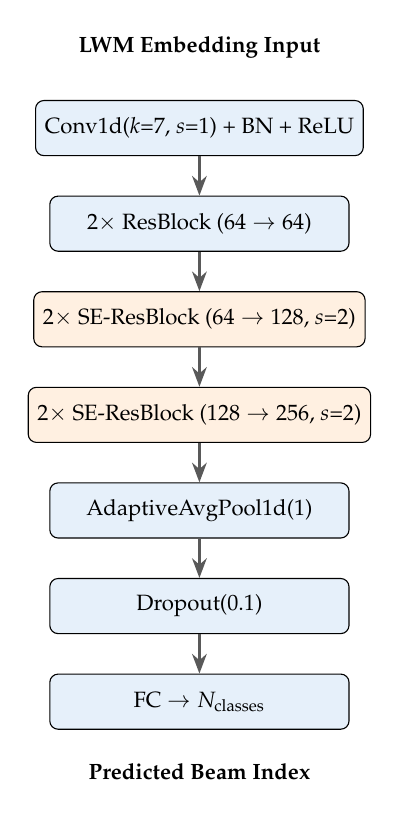
\begin{tikzpicture}[
    block/.style={rectangle, draw, fill=blockblue, minimum width=3.8cm, minimum height=0.7cm, align=center, rounded corners=3pt, font=\footnotesize},
    seb/.style={rectangle, draw, fill=blockorange, minimum width=3.8cm, minimum height=0.7cm, align=center, rounded corners=3pt, font=\footnotesize},
    arr/.style={-{Stealth[length=2.5mm]}, thick, color=gray!70!black},
    node distance=0.5cm
]
\node[block] (stem) {Conv1d($k$=7, $s$=1) + BN + ReLU};
\node[block, below=of stem] (l1) {$2\times$ ResBlock ($64 \to 64$)};
\node[seb, below=of l1] (l2) {$2\times$ SE-ResBlock ($64 \to 128$, $s$=2)};
\node[seb, below=of l2] (l3) {$2\times$ SE-ResBlock ($128 \to 256$, $s$=2)};
\node[block, below=of l3] (pool) {AdaptiveAvgPool1d(1)};
\node[block, below=of pool] (drop) {Dropout(0.1)};
\node[block, below=of drop] (fc) {FC $\to N_{\text{classes}}$};

\draw[arr] (stem) -- (l1);
\draw[arr] (l1) -- (l2);
\draw[arr] (l2) -- (l3);
\draw[arr] (l3) -- (pool);
\draw[arr] (pool) -- (drop);
\draw[arr] (drop) -- (fc);

\node[above=0.4cm of stem, font=\footnotesize\bfseries] {LWM Embedding Input};
\node[below=0.3cm of fc, font=\footnotesize\bfseries] {Predicted Beam Index};
\end{tikzpicture}
\caption{SECNN (SEResNet1D) architecture.}
\label{fig:secnn_arch}
\end{minipage}\hfill
\begin{minipage}[c]{0.52\textwidth}
\centering
\captionof{table}{Side-by-side comparison of ResCNN and SECNN design choices.}
\label{tab:arch_diff}
\resizebox{\linewidth}{!}{
\begin{tabular}{@{}lcc@{}}
\toprule
\textbf{Design Choice} & \textbf{ResCNN} & \textbf{SECNN} \\
\midrule
Stem stride            & 2 (+ MaxPool)   & 1 (no pooling) \\
Initial channel width  & 32              & 64 \\
Blocks per stage       & 2, 3, 4         & 2, 2, 2 \\
Channel widths         & 32, 64, 128     & 64, 128, 256 \\
SE attention           & None            & Layers 2 \& 3 \\
FC layers after pool   & 2 ($128 \to 65$)& 1 ($256 \to 65$) \\
Dropout rate           & 0.5             & 0.1 \\
\bottomrule
\end{tabular}
}
\end{minipage}
\end{figure}

\subsection{Training Setup}

Both models are trained under identical conditions to ensure a fair comparison.  The Adam optimiser is used with an initial learning rate of $10^{-3}$.  A MultiStepLR scheduler reduces the learning rate by a factor of $\gamma=0.1$ at epochs 15 and 35.  The loss function is standard cross-entropy, and gradient norms are clipped to a maximum of 1.0 to stabilise training.  Each configuration is trained for 30 epochs with a batch size of 32.  The full dataset of 519\,636 samples from 19 DeepMIMO city scenarios is used, with experiments repeated at six split ratios as described in Section~\ref{subsec:eval}.

\subsection{Results and Discussion}\label{subsec:results}

Table~\ref{tab:combined_results} reports the test F1 scores using both CLS ($\mathrm{emb}_{cls}$) and channel ($\mathrm{emb}_{channel}$) embeddings across six split ratios.

\begin{table}[H]
\centering
\caption{Test F1 scores on beam prediction. $\Delta$ denotes the SECNN improvement in percentage points (pp).}
\label{tab:combined_results}
\resizebox{\textwidth}{!}{
\begin{tabular}{@{}lcccccc|cccccc@{}}
\toprule
 & \multicolumn{6}{c}{\textbf{CLS Embedding ($\mathbb{R}^{64}$)}} & \multicolumn{6}{c}{\textbf{Channel Embedding ($\mathbb{R}^{128\times 64}$)}} \\
\cmidrule(lr){2-7} \cmidrule(l){8-13}
\textbf{Ratio ($r$)} & \textbf{0.5\%} & \textbf{1\%} & \textbf{5\%} & \textbf{10\%} & \textbf{20\%} & \textbf{40\%} & \textbf{0.5\%} & \textbf{1\%} & \textbf{5\%} & \textbf{10\%} & \textbf{20\%} & \textbf{40\%} \\
\midrule
ResCNN & 0.4231 & 0.5108 & 0.6642 & 0.7200 & 0.7609 & 0.8031 & 0.7815 & 0.8361 & 0.9082 & 0.9296 & 0.9394 & 0.9524 \\
SECNN  & 0.4726 & 0.5493 & 0.7098 & 0.7596 & 0.8012 & 0.8354 & 0.7810 & 0.8496 & 0.9226 & 0.9384 & 0.9508 & 0.9602 \\
$\Delta$ (pp) & \textbf{+4.95} & \textbf{+3.85} & \textbf{+4.56} & \textbf{+3.96} & \textbf{+4.03} & \textbf{+3.23} & $-$0.05 & \textbf{+1.35} & \textbf{+1.44} & \textbf{+0.88} & \textbf{+1.14} & \textbf{+0.78} \\
\bottomrule
\end{tabular}}
\end{table}

With CLS embeddings, SECNN consistently outperforms ResCNN, demonstrating a substantial average gain of $\sim$4.1\,pp. The most significant improvement (+4.95\,pp) occurs at the extreme low-data regime ($r=0.005$), highlighting the SE mechanism's ability to efficiently extract discriminative features from a compact global summary. For the spatially-resolved channel embeddings, performance is generally higher, and SECNN maintains a consistent edge (average $\sim$0.9\,pp), peaking at 0.9602 F1 score for $r=0.4$. The reduced margin compared to the CLS setting is expected, as the channel embedding already carries rich spatial structure, leaving less room for the downstream head's inductive bias to make a difference. 

\begin{figure}[H]
\centering
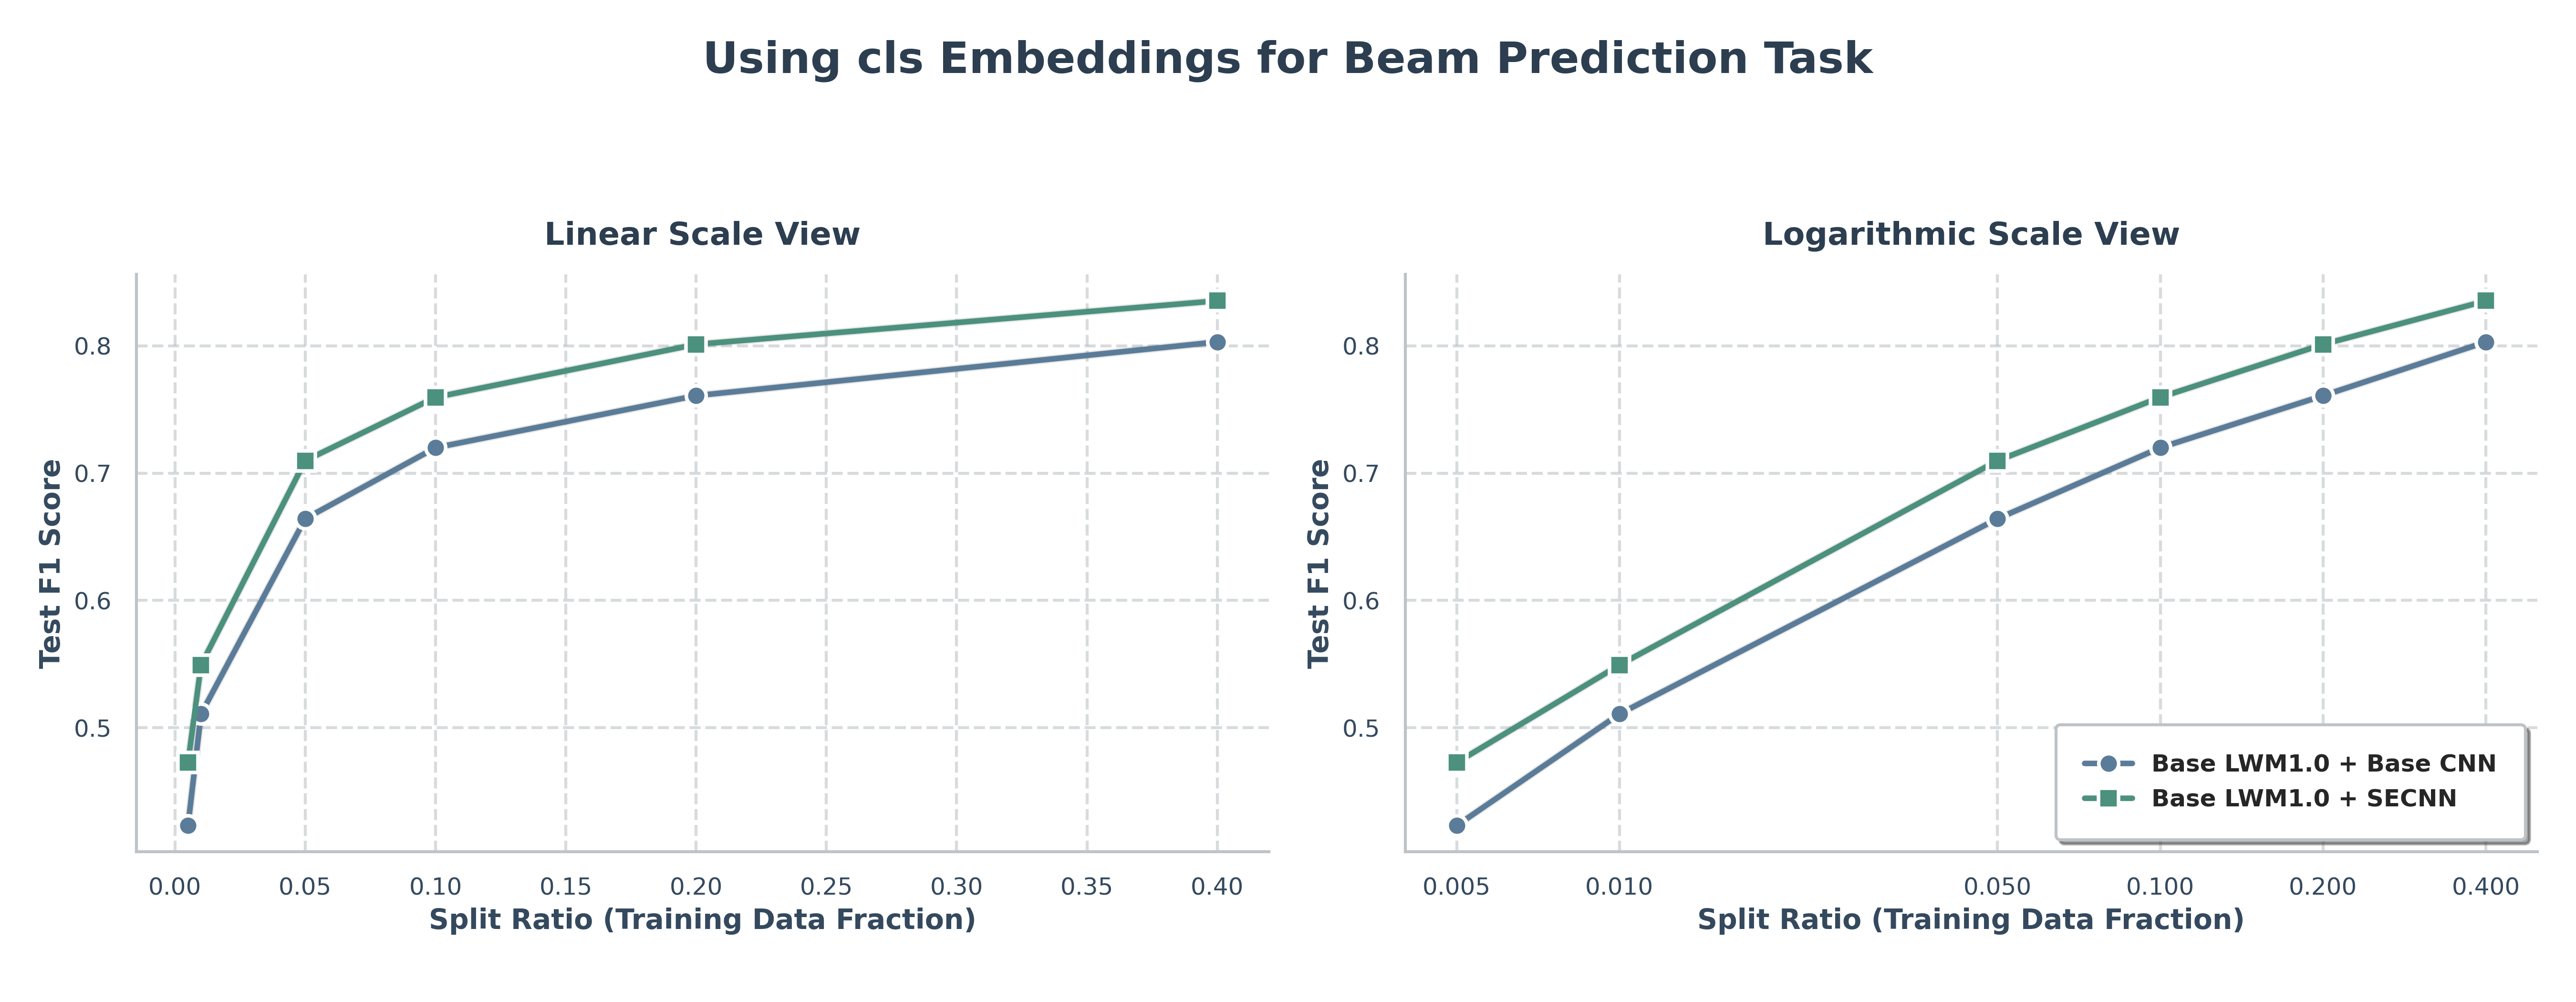
\includegraphics[width=1\textwidth]{result_photos/rescnn_vs_secnn_cls.png}
\end{figure}

\vspace{1.5em}
\begin{figure}[H]
\centering
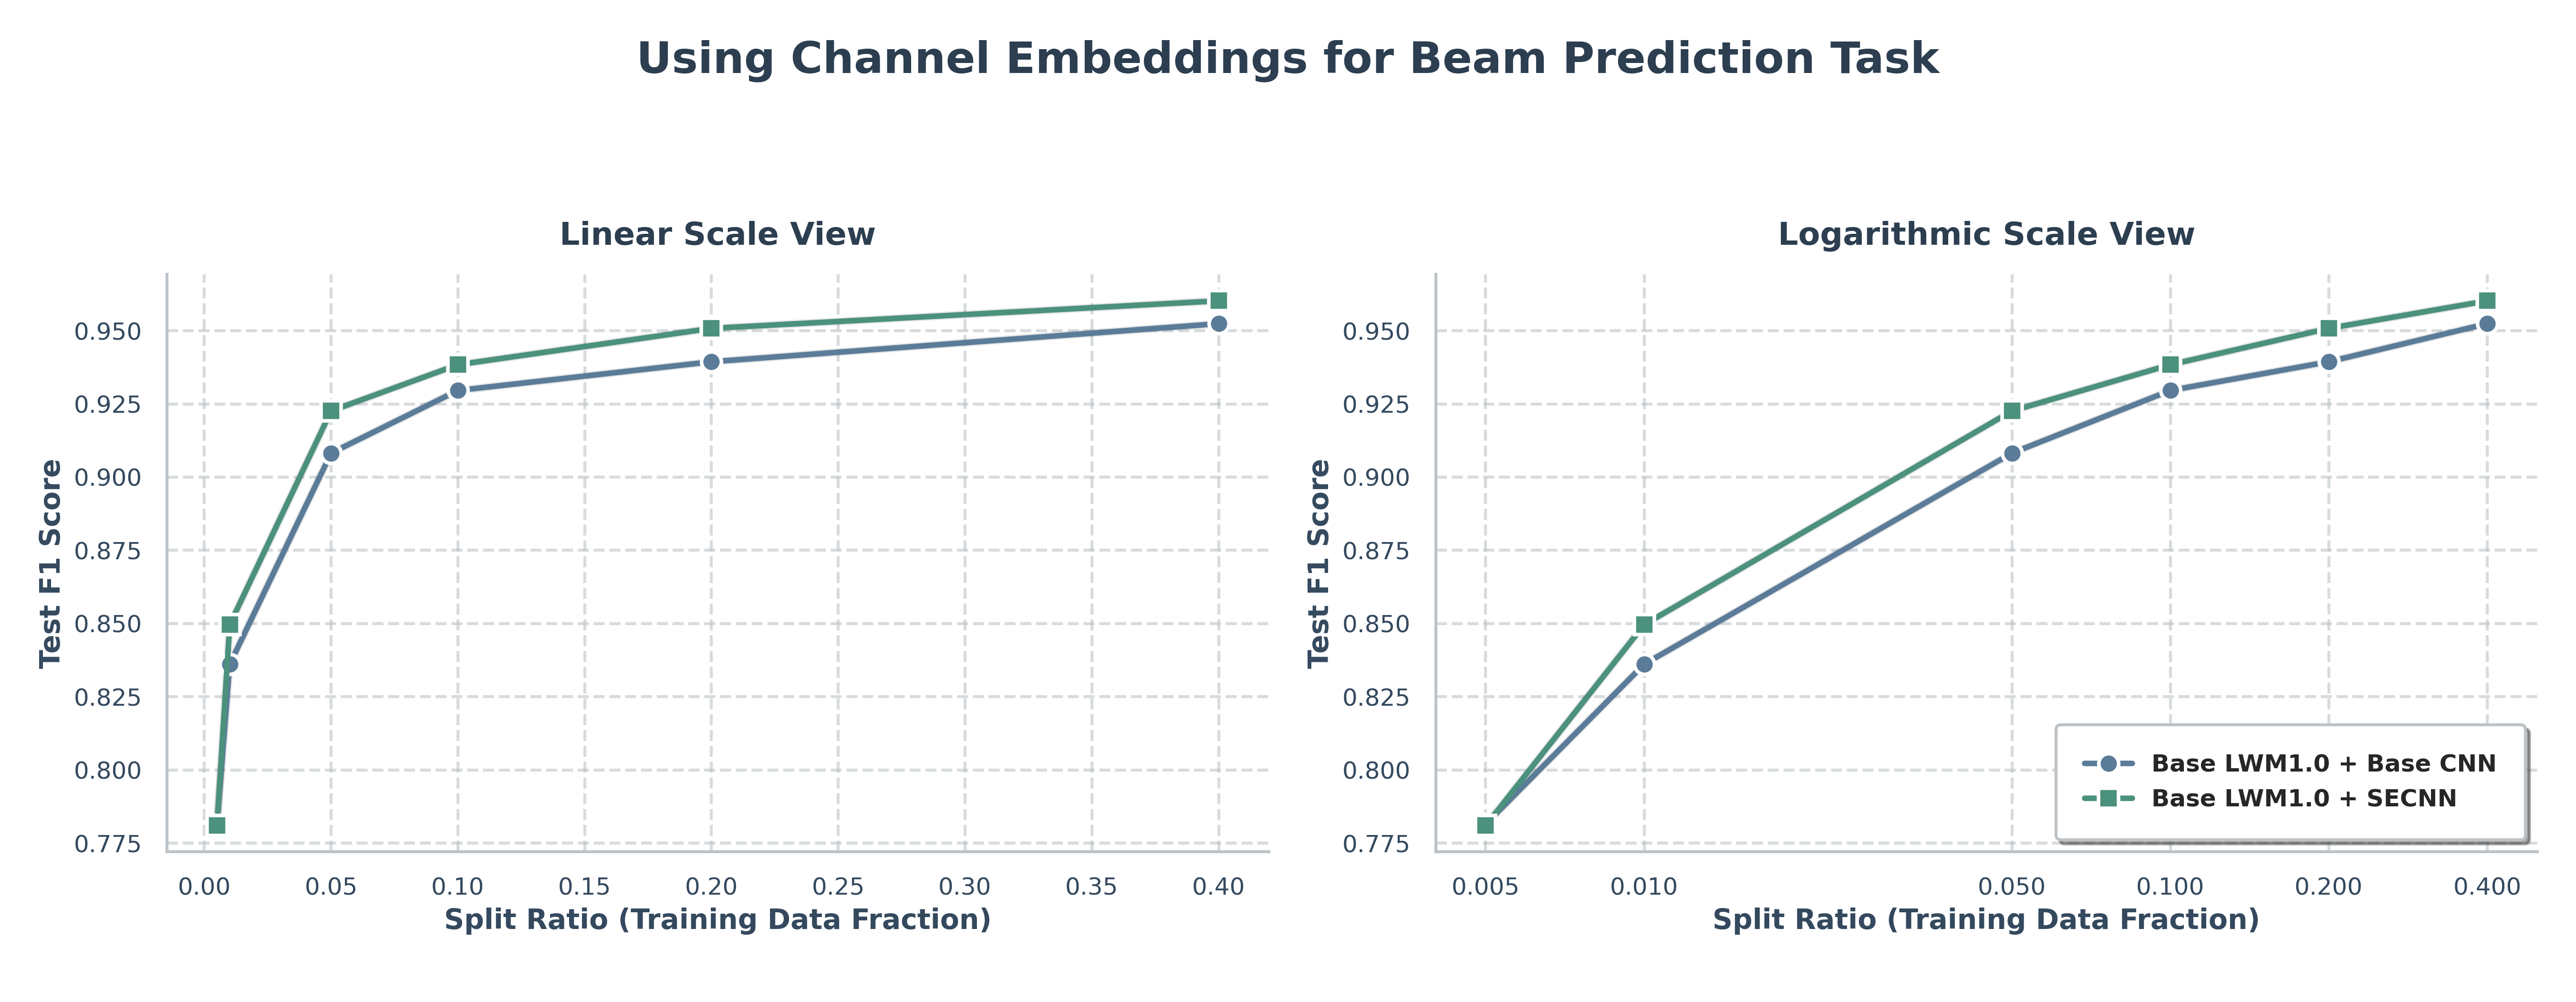
\includegraphics[width=1\textwidth]{result_photos/rescnn_vs_secnn_channel.png}
\caption{Beam prediction F1 scores. Top: CLS Embeddings. Bottom: Channel Embeddings. SECNN uniformly dominates ResCNN, especially with CLS embeddings.}
\label{fig:combined_results}
\end{figure}

\paragraph{Inferences.} Table~\ref{tab:combined_results} highlights that SECNN consistently outperforms ResCNN, with the most significant margin in the low-data regime ($r \le 0.01$). This underscores the SECNN's superior feature selection capabilities. By using a stride-1 stem without max-pooling, SECNN maintains a high-fidelity representation of the sparse wireless channel features from the very first layer. This preservation of spatial resolution, combined with the SE module's ability to "re-calibrate" and focus on discriminative channels, prevents the model from being overwhelmed by noise in the initial LWM embeddings. Furthermore, the reduction in dropout from 0.5 to 0.1 indicates that SECNN's architecture provides a more effective inductive bias, reducing the need for aggressive stochastic regularization which often leads to underfitting in small-scale wireless datasets.

\subsection{Codebase}\label{subsec:code}

The implementation for Phase~1 is contained within the \texttt{lwm/} directory. These scripts are designed for downstream beam prediction training and inference, utilizing the frozen LWM encoder as a feature extractor. The core logic is distributed as follows:

\begin{itemize}
    \item \texttt{BP\_LWM\_CNNoSECNN.py}: The primary execution script for downstream training. It defines the \texttt{res1dcnn} and \texttt{SEResNet1D} (SECNN) architectures and manages training/evaluation using embeddings extracted from the frozen LWM.
    \item \texttt{lwm\_model.py}: Defines the transformer-based LWM\,1.0 encoder.
    \item \texttt{inference.py}: Handles the forward pass of the frozen LWM backbone to extract channel embeddings, caching results in \texttt{.downstream\_cache/}.
    \item \texttt{input\_preprocess.py}: Manages DeepMIMO data parsing and beam label generation.
    \item \texttt{plotResults.py}: Generates performance plots from \texttt{results.txt}.
\end{itemize}

% ══════════════════════════════════════════════════════════════
%  4. PHASE 2: ATTENTION INTEGRATION IN LWM 1.0
% ══════════════════════════════════════════════════════════════
\newpage
\section{Phase 2: Attention Integration in LWM 1.0}\label{sec:phase2}

The second phase of the project explores improving the feature extraction capability of the LWM backbone by integrating specialized attention mechanisms. While the vanilla Multi-Head Self-Attention (MHSA) in LWM 1.0 is effective at capturing global dependencies, it treats the input as a flattened sequence, potentially ignoring the inherent 2-D structural relationships (spatial and spectral) present in wireless channels. We integrate three distinct attention paradigms: \emph{Coordinate Attention}, \emph{Axial Attention}, and \emph{Physics-guided Attention}.

\subsection{Coordinate Attention (CA)}\label{subsec:ca}

Coordinate Attention is designed to capture long-range dependencies with precise positional information. Unlike channel attention (like SE) which globalizes spatial information, CA encodes both inter-channel and position-specific information by factorizing 2-D pooling into two 1-D encoding processes.

\paragraph{Mathematical Formulation.}
Given an input feature map $\mathbf{X} \in \mathbb{R}^{C \times H \times W}$ (where $H$ and $W$ correspond to the antenna and frequency dimensions respectively), the process involves:
\begin{enumerate}
    \item \textbf{Coordinate Squeeze:} Global average pooling is performed along the horizontal and vertical axes separately:
    \begin{equation}
        z_c^h(h) = \frac{1}{W} \sum_{0 \le i < W} x_c(h, i), \quad z_c^w(w) = \frac{1}{H} \sum_{0 \le j < H} x_c(j, w)
    \end{equation}
    \item \textbf{Coordinate Excitation:} The resulting descriptors are concatenated and processed by a shared $1 \times 1$ convolution $\mathbf{F}_1$ and non-linear activation $\delta$:
    \begin{equation}
        \mathbf{f} = \delta(\mathbf{F}_1([\mathbf{z}^h, \mathbf{z}^w]))
    \end{equation}
    where $[\cdot, \cdot]$ denotes concatenation along the spatial dimension. $\mathbf{f} \in \mathbb{R}^{C/r \times (H+W)}$ is then split back into $\mathbf{f}^h \in \mathbb{R}^{C/r \times H}$ and $\mathbf{f}^w \in \mathbb{R}^{C/r \times W}$.
    \item \textbf{Recalibration:} Two $1 \times 1$ convolutions $\mathbf{F}_h$ and $\mathbf{F}_w$ transform $\mathbf{f}^h$ and $\mathbf{f}^w$ back to the original channel dimension, followed by a sigmoid $\sigma$ to produce attention weights:
    \begin{equation}
        g_c^h = \sigma(\mathbf{F}_h(\mathbf{f}^h)), \quad g_c^w = \sigma(\mathbf{F}_w(\mathbf{f}^w))
    \end{equation}
    The final output is $\tilde{x}_c(i, j) = x_c(i, j) \times g_c^h(i) \times g_c^w(j)$.
\end{enumerate}

\begin{figure}[H]
\centering
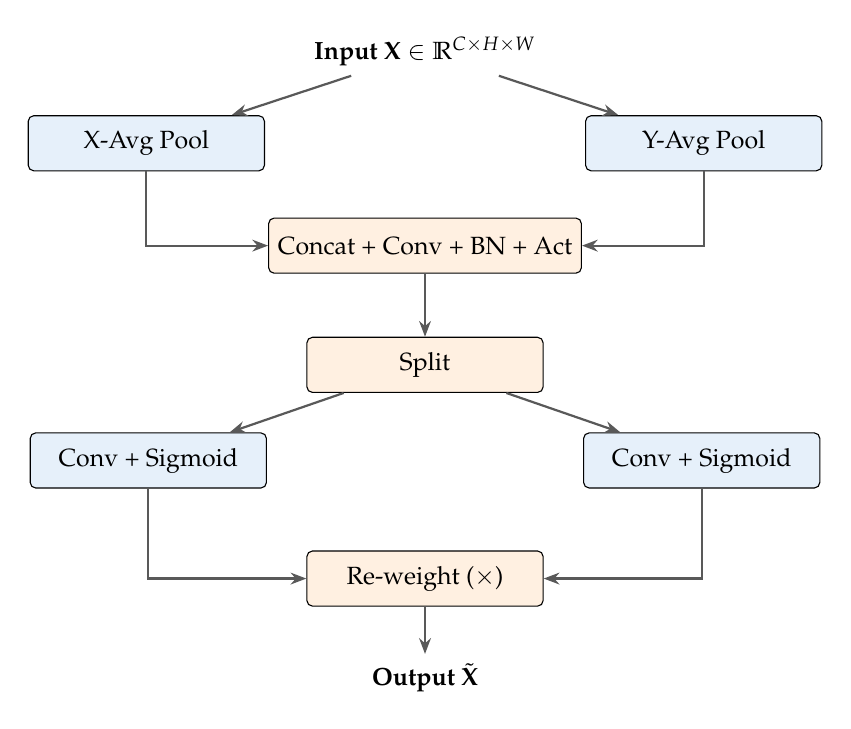
\begin{tikzpicture}[
    node distance=0.8cm,
    block/.style={rectangle, draw, fill=blockblue, minimum width=3cm, minimum height=0.7cm, align=center, rounded corners=2pt, font=\small},
    proc/.style={rectangle, draw, fill=blockorange, minimum width=3cm, minimum height=0.7cm, align=center, rounded corners=2pt, font=\small},
    arr/.style={-{Stealth[length=2mm]}, thick, color=gray!70!black}
]
    \node (inp) [font=\small\bfseries] {Input $\mathbf{X} \in \mathbb{R}^{C \times H \times W}$};
    \node (poolh) [block, below left=0.5cm and 0.5cm of inp] {X-Avg Pool};
    \node (poolw) [block, below right=0.5cm and 0.5cm of inp] {Y-Avg Pool};
    \node (cat) [proc, below=1.8cm of inp] {Concat + Conv + BN + Act};
    \node (split) [proc, below=0.8cm of cat] {Split};
    \node (convh) [block, below left=0.5cm and 0.5cm of split] {Conv + Sigmoid};
    \node (convw) [block, below right=0.5cm and 0.5cm of split] {Conv + Sigmoid};
    \node (mul) [proc, below=2cm of split] {Re-weight ($\times$)};
    \node (out) [below=0.6cm of mul, font=\small\bfseries] {Output $\tilde{\mathbf{X}}$};

    \draw[arr] (inp) -- (poolh);
    \draw[arr] (inp) -- (poolw);
    \draw[arr] (poolh) |- (cat);
    \draw[arr] (poolw) |- (cat);
    \draw[arr] (cat) -- (split);
    \draw[arr] (split) -- (convh);
    \draw[arr] (split) -- (convw);
    \draw[arr] (convh) |- (mul);
    \draw[arr] (convw) |- (mul);
    \draw[arr] (mul) -- (out);
\end{tikzpicture}
\caption{Coordinate Attention mechanism. It factorizes 2D pooling into two 1D encoding processes to capture direction-aware and position-sensitive information.}
\label{fig:coord_att}
\end{figure}

\subsection{Axial Attention}\label{subsec:axial}

Axial Attention reduces the computational burden of global attention by factorizing it into sequential 1-D attention operations along the different axes of the input. In LWM, this means performing attention separately across the antenna dimension ($H=32$) and the frequency dimension ($W=4$).

\paragraph{Mathematical Formulation.}
For an input grid $\mathbf{X} \in \mathbb{R}^{H \times W \times D}$, axial attention computes:
\begin{enumerate}
    \item \textbf{Antenna-axis Attention:} Fixes the frequency index $j$ and performs MHSA over the antenna index $i$:
    \begin{equation}
        \mathbf{Y}_{i,j}^{ant} = \text{MHSA}_{i}(\mathbf{X}_{i,j}) + \mathbf{X}_{i,j}
    \end{equation}
    \item \textbf{Frequency-axis Attention:} Fixes the antenna index $i$ and performs MHSA over the frequency index $j$:
    \begin{equation}
        \mathbf{Y}_{i,j}^{freq} = \text{MHSA}_{j}(\mathbf{Y}_{i,j}^{ant}) + \mathbf{Y}_{i,j}^{ant}
    \end{equation}
\end{enumerate}
This reduces complexity from $O((H \cdot W)^2)$ to $O(H \cdot W(H+W))$, which is particularly beneficial for high-resolution channel grids. Furthermore, we incorporate \textbf{Rotary Positional Embeddings (RoPE)} within each axial operation to inject relative positional information into the attention scores, allowing the model to distinguish between different spatial and spectral lags.

\subsection{Physics-guided Attention}\label{subsec:physics}

Physics-guided attention leverages the underlying physical properties of wireless channels—specifically spatial correlation and frequency coherence—to bias the self-attention mechanism towards physically meaningful relationships.

\paragraph{Physical Prior Bias.}
We construct a bias matrix $\mathbf{\Phi} \in \mathbb{R}^{S \times S}$ (where $S = HW+1$) that encodes the expected correlation between tokens based on their spatial and spectral distances:
\begin{equation}
    \Phi_{i,j} = \exp\left(-\frac{|ant_i - ant_j|^2}{2\sigma^2}\right) \cdot \exp\left(-\frac{|freq_i - freq_j|}{\tau_c}\right)
\end{equation}
where $ant_i$ and $freq_i$ are the antenna and frequency indices of token $i$ respectively. The first term represents the spatial decay over the antenna array, while the second term captures frequency selectivity.

\paragraph{Modified Attention Score.}
The physics prior is integrated as an additive bias to the attention logits before the softmax operation:
\begin{equation}
    \text{Attn}(\mathbf{Q}, \mathbf{K}, \mathbf{V}) = \text{Softmax}\left(\frac{\mathbf{QK}^T}{\sqrt{d_k}} + \lambda \mathbf{\Phi}\right)\mathbf{V}
\end{equation}
where $\lambda$ is a learnable scaling factor. This bias encourages the model to focus on clusters of patches that are physically adjacent, reflecting the typical structure of multipath channel components.

\begin{figure}[H]
\centering
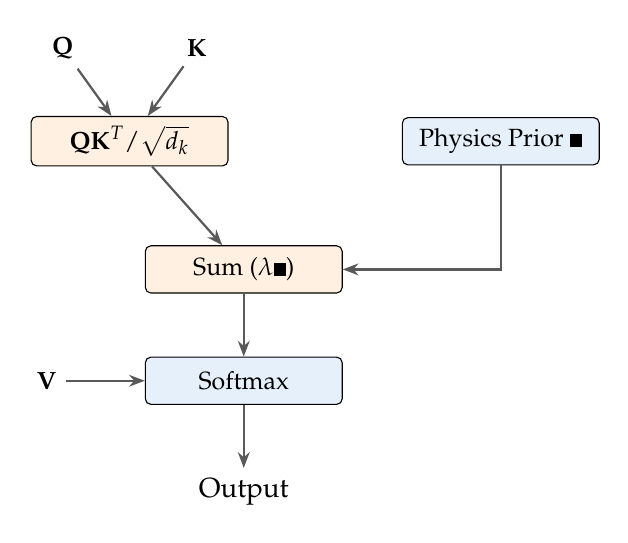
\begin{tikzpicture}[
    node distance=1cm,
    block/.style={rectangle, draw, fill=blockblue, minimum width=2.5cm, minimum height=0.6cm, align=center, rounded corners=2pt, font=\small},
    proc/.style={rectangle, draw, fill=blockorange, minimum width=2.5cm, minimum height=0.6cm, align=center, rounded corners=2pt, font=\small},
    arr/.style={-{Stealth[length=2mm]}, thick, color=gray!70!black}
]
    \node (q) [font=\small] {$\mathbf{Q}$};
    \node (k) [font=\small, right=1.2cm of q] {$\mathbf{K}$};
    \node (dot) [proc, below=0.6cm of q, xshift=0.85cm] {$\mathbf{QK}^T / \sqrt{d_k}$};
    \node (phi) [block, right=2.2cm of dot] {Physics Prior $\mathbf{\Phi}$};
    \node (sum) [proc, below=1cm of dot, xshift=1.45cm] {Sum ($\lambda \mathbf{\Phi}$)};
    \node (soft) [block, below=0.8cm of sum] {Softmax};
    \node (v) [font=\small, left=1cm of soft] {$\mathbf{V}$};
    \node (out) [below=0.8cm of soft] {Output};

    \draw[arr] (q) -- (dot);
    \draw[arr] (k) -- (dot);
    \draw[arr] (dot) -- (sum);
    \draw[arr] (phi) |- (sum);
    \draw[arr] (sum) -- (soft);
    \draw[arr] (v) -- (soft);
    \draw[arr] (soft) -- (out);
\end{tikzpicture}
\caption{Physics-guided Attention. A physics-derived bias matrix $\mathbf{\Phi}$ is added to the attention scores to emphasize spatial and spectral locality.}
\label{fig:physics_att}
\end{figure}

\subsection{Results and Discussion}\label{subsec:results_p2}

\paragraph{Inferences.} Several key insights emerge from the attention variants comparison. First, the superiority of \textbf{Coordinate Attention (CA)} on channel embeddings is attributed to its ability to encode precise positional information through direction-aware pooling. Unlike global SE attention which flattens spatial structure, CA factorizes 2D pooling into separate antenna and frequency descriptors, allowing the shared $1 \times 1$ convolution to capture inter-dimensional dependencies. This is critical for the 128x64 channel grid where spatial-spectral locality is a dominant feature.

Second, \textbf{Axial Attention}'s peak performance at the 0.5\% CLS split (0.6756 vs 0.5805 for CA) suggests that its factored MHSA structure acts as a powerful regularizer. By decomposing the global attention into separate antenna and frequency passes, Axial attention significantly reduces the search space for the model, providing a strong structural bias that prevents overfitting when training labels are extremely sparse. Finally, the performance of \textbf{Physics-guided Attention} confirms that while physical priors (spatial/spectral decay) provide a solid performance floor, they are ultimately surpassed by data-driven mechanisms like CA that can learn to account for non-idealized channel propagation, such as diffraction and scattering, which are not perfectly captured by the exponential decay prior.

\begin{table}[H]
\centering
\caption{Test F1 scores on beam prediction with integrated attention mechanisms.}
\label{tab:results_p2}
\resizebox{\textwidth}{!}{
\begin{tabular}{@{}lcccccc|cccccc@{}}
\toprule
 & \multicolumn{6}{c}{\textbf{CLS Embedding ($\mathbb{R}^{64}$)}} & \multicolumn{6}{c}{\textbf{Channel Embedding ($\mathbb{R}^{128\times 64}$)}} \\
\cmidrule(lr){2-7} \cmidrule(l){8-13}
\textbf{Ratio ($r$)} & \textbf{0.5\%} & \textbf{1\%} & \textbf{5\%} & \textbf{10\%} & \textbf{20\%} & \textbf{40\%} & \textbf{0.5\%} & \textbf{1\%} & \textbf{5\%} & \textbf{10\%} & \textbf{20\%} & \textbf{40\%} \\
\midrule
LWM\_Axial & \textbf{0.6756} & \textbf{0.7251} & \textbf{0.8000} & 0.8185 & 0.8318 & 0.8407 & 0.6978 & 0.7572 & 0.8923 & 0.9139 & 0.9295 & 0.9402 \\
LWM\_CA    & 0.5805 & 0.6601 & 0.7959 & \textbf{0.8351} & \textbf{0.8576} & \textbf{0.8748} & \textbf{0.8196} & \textbf{0.8694} & \textbf{0.9287} & \textbf{0.9410} & \textbf{0.9525} & \textbf{0.9592} \\
LWM\_Phys  & 0.6056 & 0.6692 & 0.7639 & 0.7884 & 0.8028 & 0.8141 & 0.7275 & 0.8025 & 0.8979 & 0.9239 & 0.9363 & 0.9451 \\
\bottomrule
\end{tabular}}
\end{table}

\begin{figure}[H]
\centering
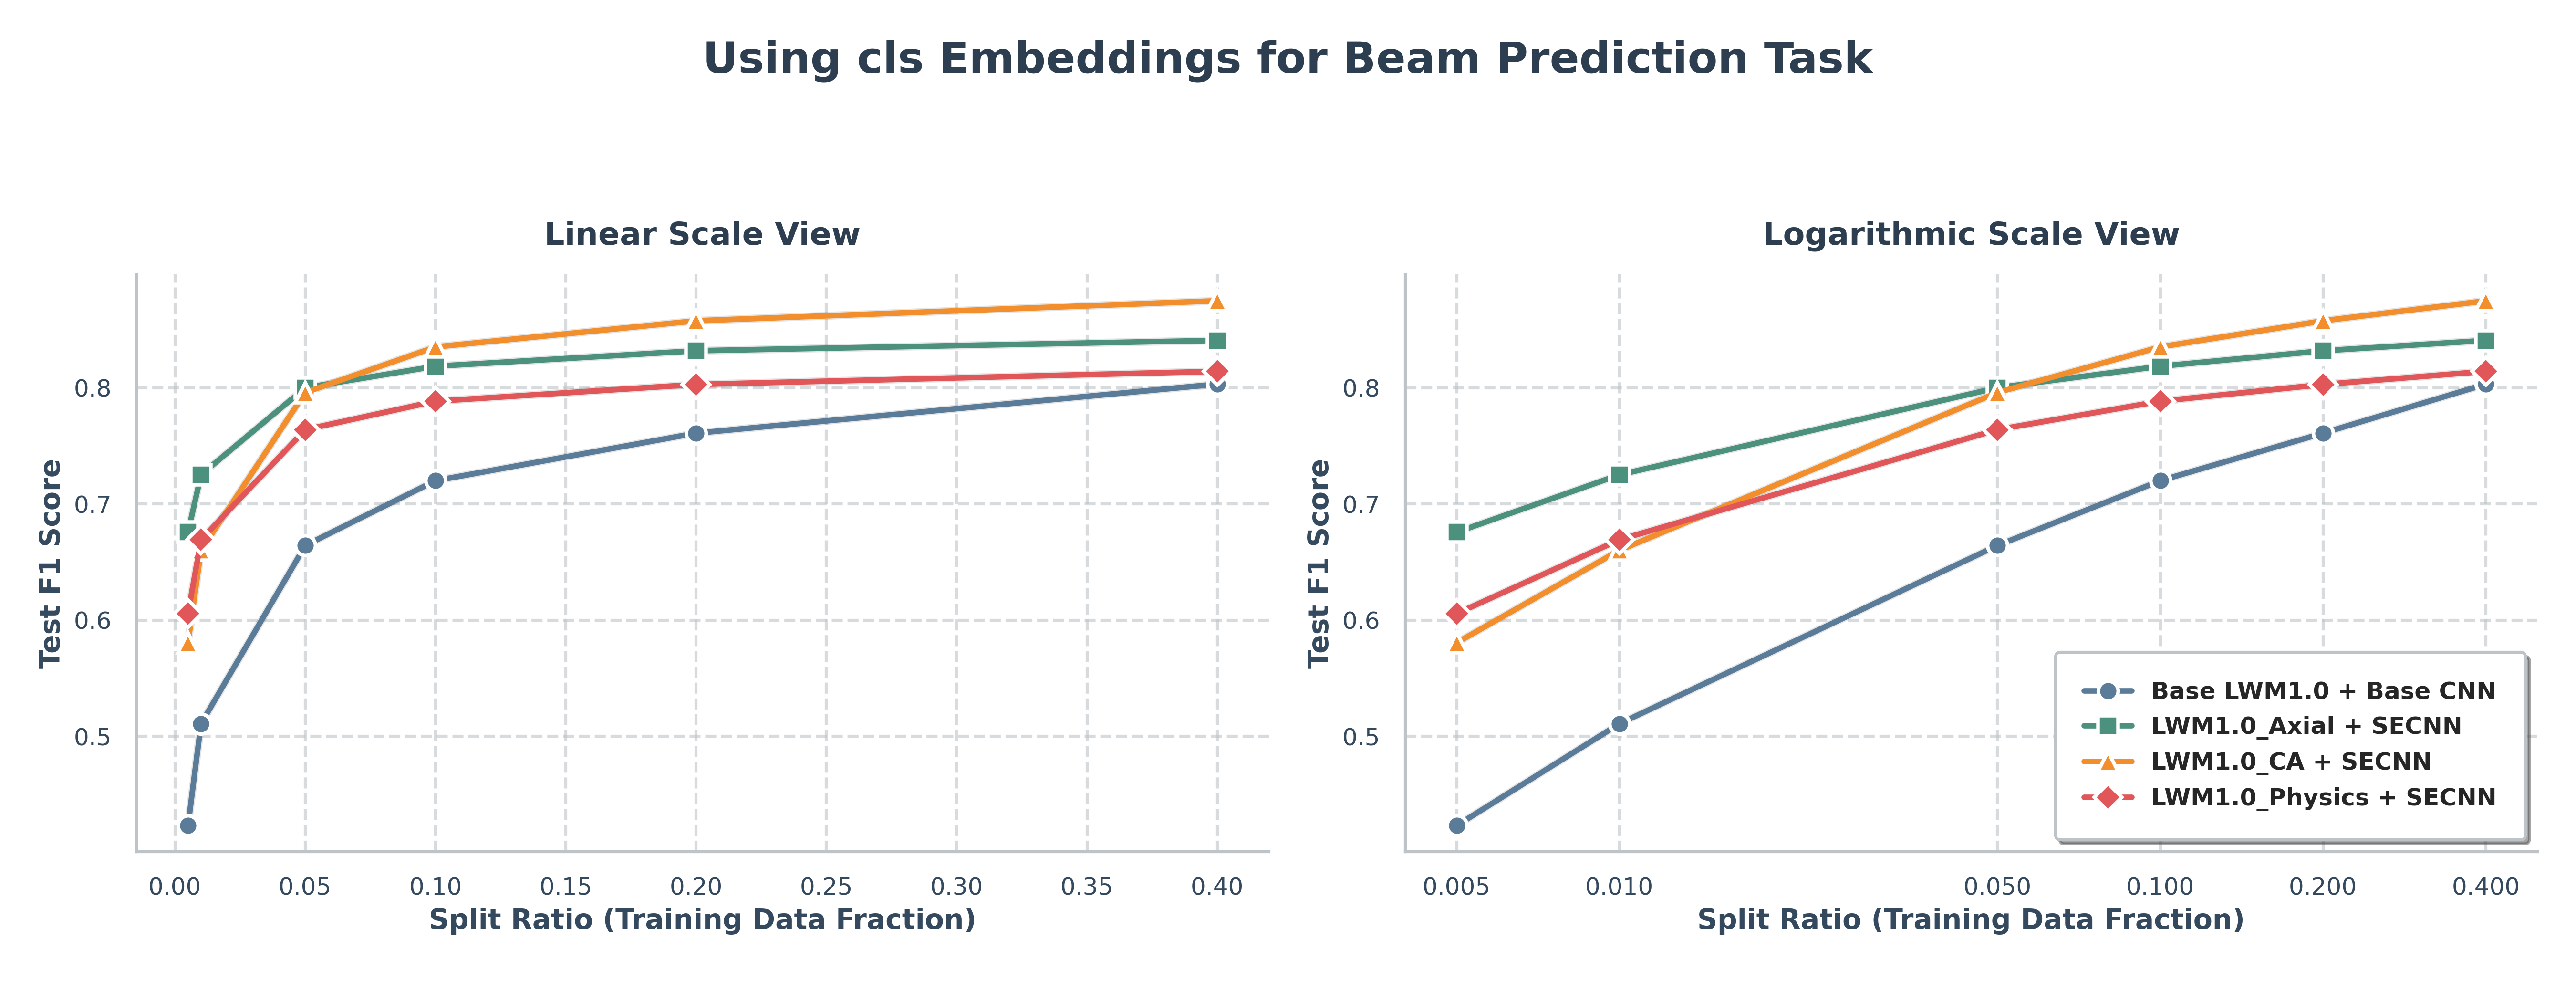
\includegraphics[width=1\textwidth]{result_photos/lwm_axial_ca_phy_cls.png}
\end{figure}

\vspace{1.5em}
\begin{figure}[H]
\centering
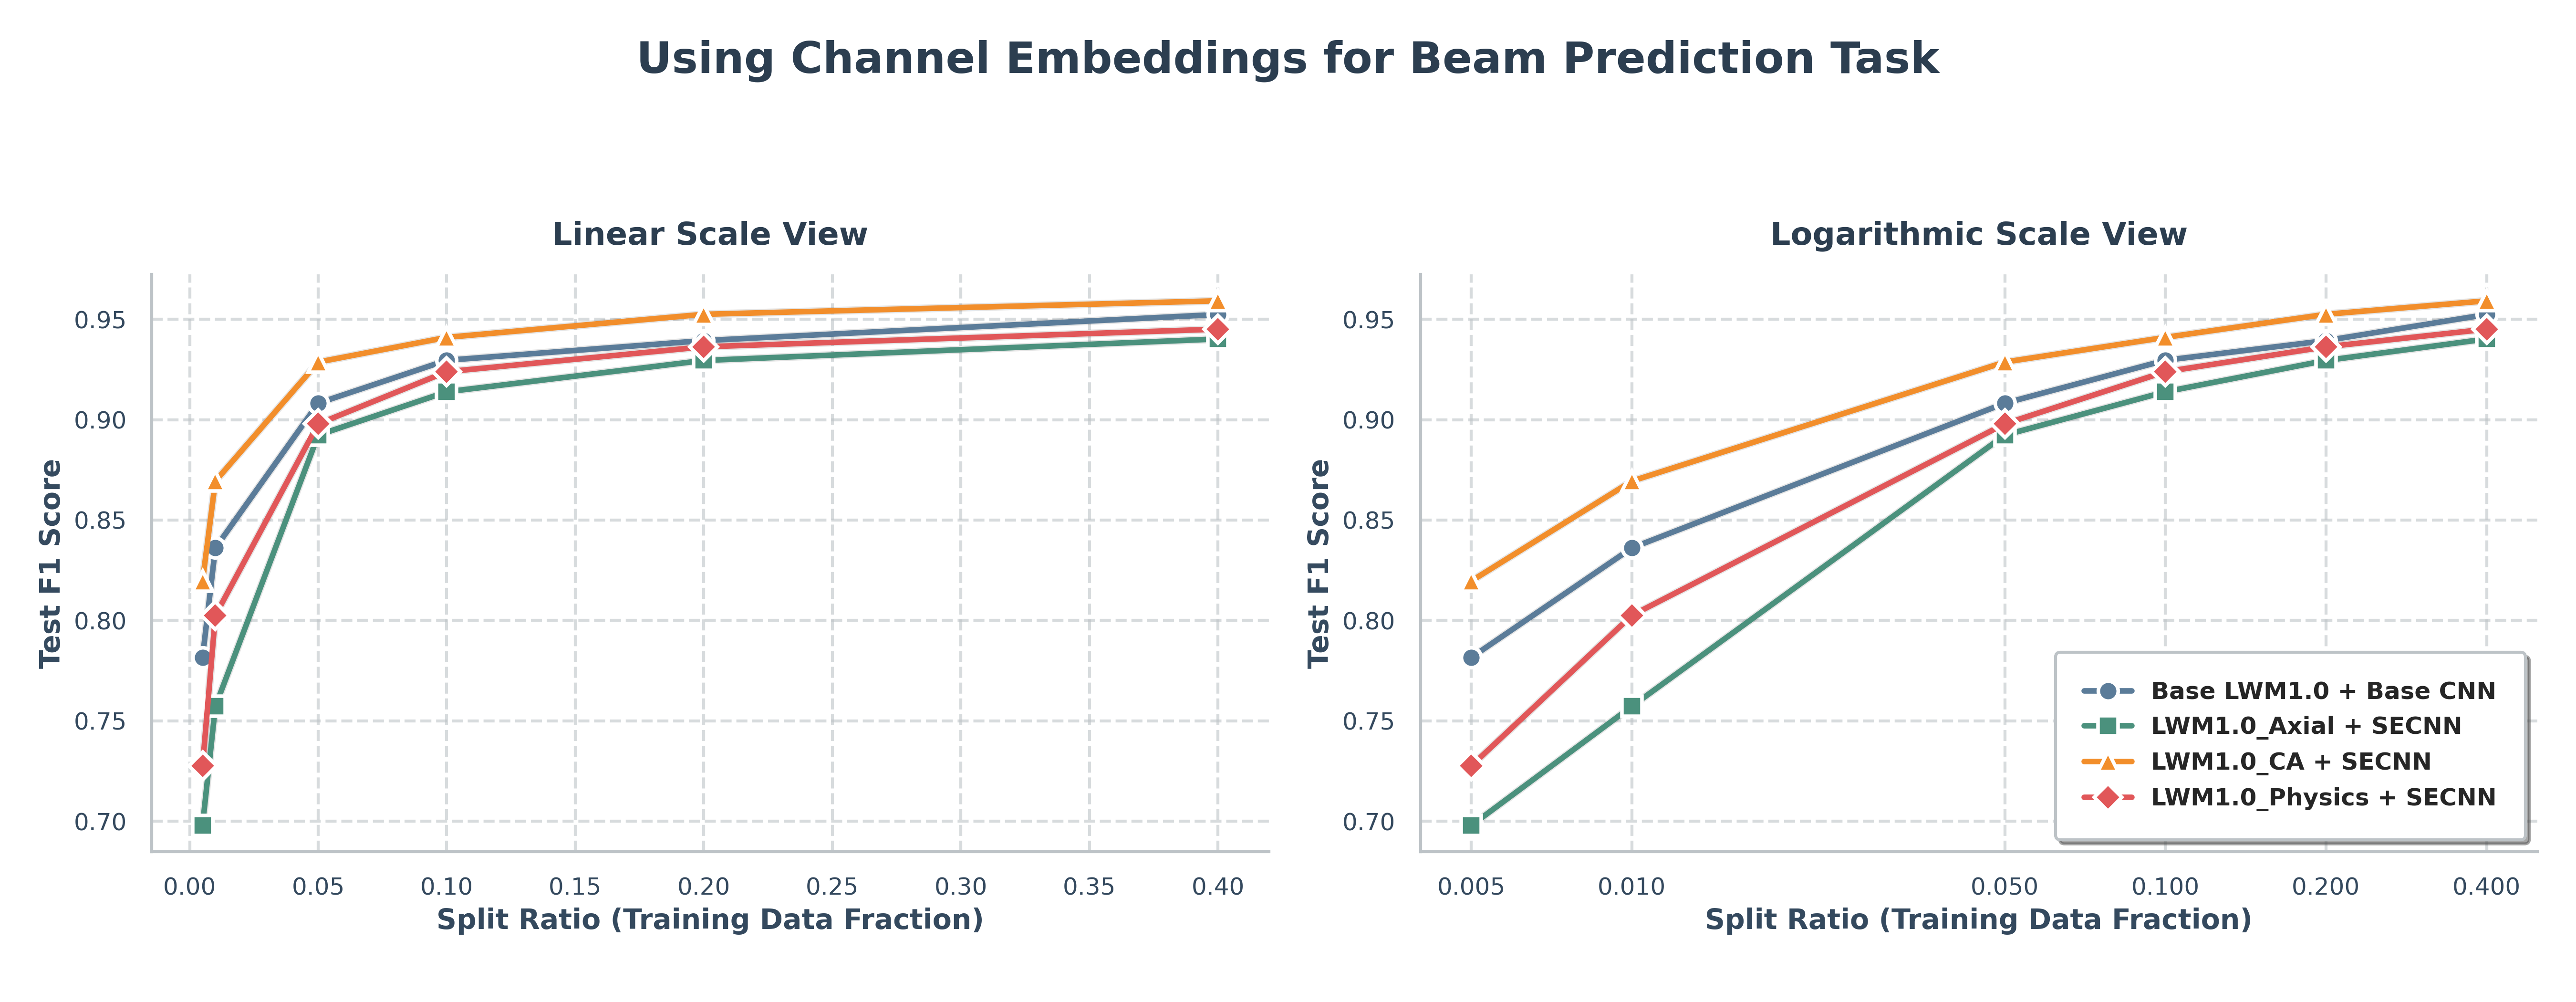
\includegraphics[width=1\textwidth]{result_photos/lwm_axial_ca_phy_channel.png}
\caption{Beam prediction performance comparison for Phase 2 attention variants. Top: CLS Embeddings. Bottom: Channel Embeddings.}
\label{fig:results_p2}
\end{figure}

\subsection{Codebase}\label{subsec:code_p2}

Phase~2 development is modularized into three separate folders. Each contains specialized scripts for downstream beam prediction training and inference, leveraging a frozen, attention-augmented LWM backbone:

\begin{itemize}[leftmargin=1.2em]
    \item \texttt{lwm\_ca/}: Contains \texttt{coordatt.py} (Coordinate Attention block). Downstream training is performed by \texttt{BP\_CA\_LWM\_SECNN.py}, which recalibrates the spatial-spectral grid before inferencing from the frozen LWM backbone.
    \item \texttt{lwm\_axial/}: Houses \texttt{axial\_linear\_att.py}. The \texttt{AxialSoftmaxAttention} module is integrated into the LWM backbone in \texttt{lwm\_axial\_model.py}. \texttt{BP\_AXL\_LWM\_SECNN.py} manages the downstream beam prediction tasks using the frozen encoder.
    \item \texttt{lwm\_physics/}: Features \texttt{physics\_priors.py} and \texttt{lwm\_physics\_model.py}. The \texttt{BP\_PHY\_LWM\_SECNN.py} script executes the benchmarking pipeline, inferencing from the physics-biased backbone.
\end{itemize}

Each directory is self-contained with its own \texttt{inference.py} and \texttt{results.txt}, with all \texttt{BP\_} scripts focusing on training the downstream head using features from the frozen encoder.

% ══════════════════════════════════════════════════════════════
%  5. PHASE 3: LWM 1.1 AND COORDINATE ATTENTION INTEGRATION
% ══════════════════════════════════════════════════════════════
\newpage
\section{Phase 3: Coordinate Attention on LWM 1.1}\label{sec:phase3}

Having established Coordinate Attention (CA) as the best-performing attention variant on LWM~1.0 (Section~\ref{sec:phase2}), Phase~3 ports this mechanism to the next-generation backbone, \textbf{LWM~1.1}~\cite{lwm11}, and benchmarks the combined system against both the vanilla LWM~1.0 and the vanilla LWM~1.1 baselines.

\subsection{LWM 1.1: Architectural Evolution}\label{subsec:improvements_p3}

LWM~1.1 addresses core limitations in scalability, model capacity, and pre-training diversity relative to version~1.0. Table~\ref{tab:lwm_comp} summarizes the key changes.

\begin{table}[H]
\centering
\caption{Comparison of LWM 1.0 and LWM 1.1 specifications.}
\label{tab:lwm_comp}
\begin{tabular}{@{}lcc@{}}
\toprule
\textbf{Feature} & \textbf{LWM 1.0} & \textbf{LWM 1.1} \\
\midrule
Channel size support     & Fixed $(32, 32)$       & Multiple $(N, SC)$ pairs \\
Max sequence length      & 128                    & \textbf{512} \\
Embedding dim ($d_{model}$) & 64                 & \textbf{128} \\
Parameters               & 600\,K                 & \textbf{2.5\,M} \\
Attention heads           & 12                     & \textbf{8} \\
MCM masking ratio        & 15\%                   & \textbf{40\%} \\
Patch segmentation       & 1-D (antenna \emph{or} freq.) & \textbf{2-D ($4{\times}4$ ant.${\times}$freq.)} \\
Pre-training samples     & 820\,K                 & \textbf{$\sim$1.3\,M} \\
Pre-training scenarios   & 15                     & \textbf{140} \\
Optimizer / schedule     & Adam                   & \textbf{AdamW + cosine decay} \\
\bottomrule
\end{tabular}
\end{table}

\paragraph{2-D Patch Segmentation.}
LWM~1.0 flattened the channel along a single axis before tokenization. LWM~1.1 introduces \textbf{2-D patches} of size $4{\times}4$ (antennas $\times$ subcarriers), producing $n_\text{patches}=64$ tokens from a $(32,32)$ grid. Each patch vector has length $4 \times 4 \times 2 = 32$ (real + imaginary), yielding a richer spatial-spectral representation that aligns naturally with OFDM channel structure.

\paragraph{Masked Channel Modelling (MCM).}
Both versions share the MCM self-supervised objective, but LWM~1.1 raises the masking ratio from 15\% to \textbf{40\%}. An 80-10-10 corruption scheme is applied (80\% \texttt{[MASK]}, 10\% random, 10\% unchanged). The loss is a variance-normalized MSE:
\begin{equation}
    \mathcal{L}_{\text{MCM}} = \frac{\text{MSE}\!\bigl(\mathbf{T}_{\text{mask}},\;\hat{\mathbf{T}}_{\text{mask}}\bigr)}{\text{Var}\!\bigl(\mathbf{T}_{\text{mask}}\bigr)}
\end{equation}
where $\mathbf{T}_{\text{mask}}$ and $\hat{\mathbf{T}}_{\text{mask}}$ are the ground-truth and predicted tokens at the masked positions. The increased masking forces the model to rely on deeper spatial-spectral correlations rather than local context, producing more robust embeddings.

\subsection{CA Integration into LWM 1.1}\label{subsec:ca_lwm11}

The Coordinate Attention block (described in Section~\ref{subsec:ca}, Figure~\ref{fig:coord_att}) is inserted \emph{before} the 2-D patching stage. The raw complex channel $\mathbf{H} \in \mathbb{R}^{2 \times 32 \times 32}$ (real and imaginary stacked) is first recalibrated by the CA module, which produces direction-aware attention maps along the antenna and subcarrier axes. The recalibrated channel is then tokenized into $4{\times}4$ patches, masked, and processed by the 12-layer LWM~1.1 transformer. This end-to-end pipeline (\texttt{torch\_pipeline\_v11.py}) is pre-trained jointly via MCM, allowing the CA weights to co-adapt with the backbone.

\subsection{Results and Discussion}\label{subsec:results_p3}

Table~\ref{tab:results_p3} reports the cross-generational comparison across all four configurations. The LWM~1.0 variants use the Base CNN and CA+SECNN heads from Phases~1 and~2 respectively; the LWM~1.1 variants mirror this pairing.

\begin{table}[H]
\centering
\caption{Generational comparison of beam prediction F1 scores.}
\label{tab:results_p3}
\resizebox{\textwidth}{!}{
\begin{tabular}{@{}lcccccc|cccccc@{}}
\toprule
 & \multicolumn{6}{c}{\textbf{CLS Embedding}} & \multicolumn{6}{c}{\textbf{Channel Embedding}} \\
\cmidrule(lr){2-7} \cmidrule(l){8-13}
\textbf{Ratio ($r$)} & \textbf{0.5\%} & \textbf{1\%} & \textbf{5\%} & \textbf{10\%} & \textbf{20\%} & \textbf{40\%} & \textbf{0.5\%} & \textbf{1\%} & \textbf{5\%} & \textbf{10\%} & \textbf{20\%} & \textbf{40\%} \\
\midrule
Base LWM 1.0 + Base CNN & 0.4231 & 0.5108 & 0.6642 & 0.7200 & 0.7609 & 0.8031 & 0.7815 & 0.8361 & 0.9082 & 0.9296 & 0.9394 & 0.9524 \\
LWM 1.0\_CA + SECNN      & 0.5805 & 0.6601 & 0.7959 & 0.8351 & 0.8576 & 0.8748 & 0.8196 & 0.8694 & 0.9287 & 0.9410 & 0.9525 & 0.9592 \\
Base LWM 1.1 + Base CNN & 0.4003 & 0.4046 & 0.5679 & 0.5758 & 0.6878 & 0.7314 & 0.7119 & 0.7905 & 0.8866 & 0.9105 & 0.9302 & 0.9454 \\
LWM 1.1\_CA + SECNN      & 0.4921 & 0.5686 & 0.7218 & 0.7632 & 0.7823 & 0.8021 & 0.7528 & 0.8164 & 0.9101 & 0.9255 & 0.9400 & 0.9480 \\
\bottomrule
\end{tabular}}
\end{table}

\paragraph{Inferences.}
\begin{enumerate}
    \item \textbf{LWM 1.0\_CA + SECNN remains the overall leader.} The Phase~2 best configuration dominates across both embedding types and all split ratios (e.g., 0.8748 CLS F1 at $r{=}0.4$). This confirms that the CA recalibration, when applied to the mature LWM~1.0 backbone with SECNN, produces the strongest downstream features in our evaluation.

    \item \textbf{LWM 1.1 underperforms LWM 1.0 at low data.} The vanilla LWM~1.1 backbone (2.5\,M parameters, 40\% masking) trails the compact LWM~1.0 (600\,K parameters, 15\% masking) across all CLS split ratios and low-data channel splits. The higher-dimensional embedding space ($d{=}128$ vs $d{=}64$) requires more downstream supervision to resolve, creating a ``cold-start'' penalty.

    \item \textbf{CA recovers LWM 1.1 to competitive levels.} Applying Coordinate Attention to LWM~1.1 yields large gains over the vanilla 1.1 baseline --- +9.2\,pp at $r{=}0.005$ and +16.4\,pp at $r{=}0.01$ on CLS embeddings. While it does not surpass LWM~1.0\_CA, it closes the gap substantially, demonstrating that CA's directional priors are essential for unlocking the potential of the larger backbone in low-data regimes.

    \item \textbf{Channel embeddings converge across generations.} For channel embeddings at $r \ge 0.05$, all four models converge to within ${\sim}2$\,pp (0.91--0.96 F1), indicating that the spatial richness of high-dimensional channel embeddings saturates the downstream head regardless of the backbone or attention variant used.
\end{enumerate}


\begin{figure}[H]
\centering
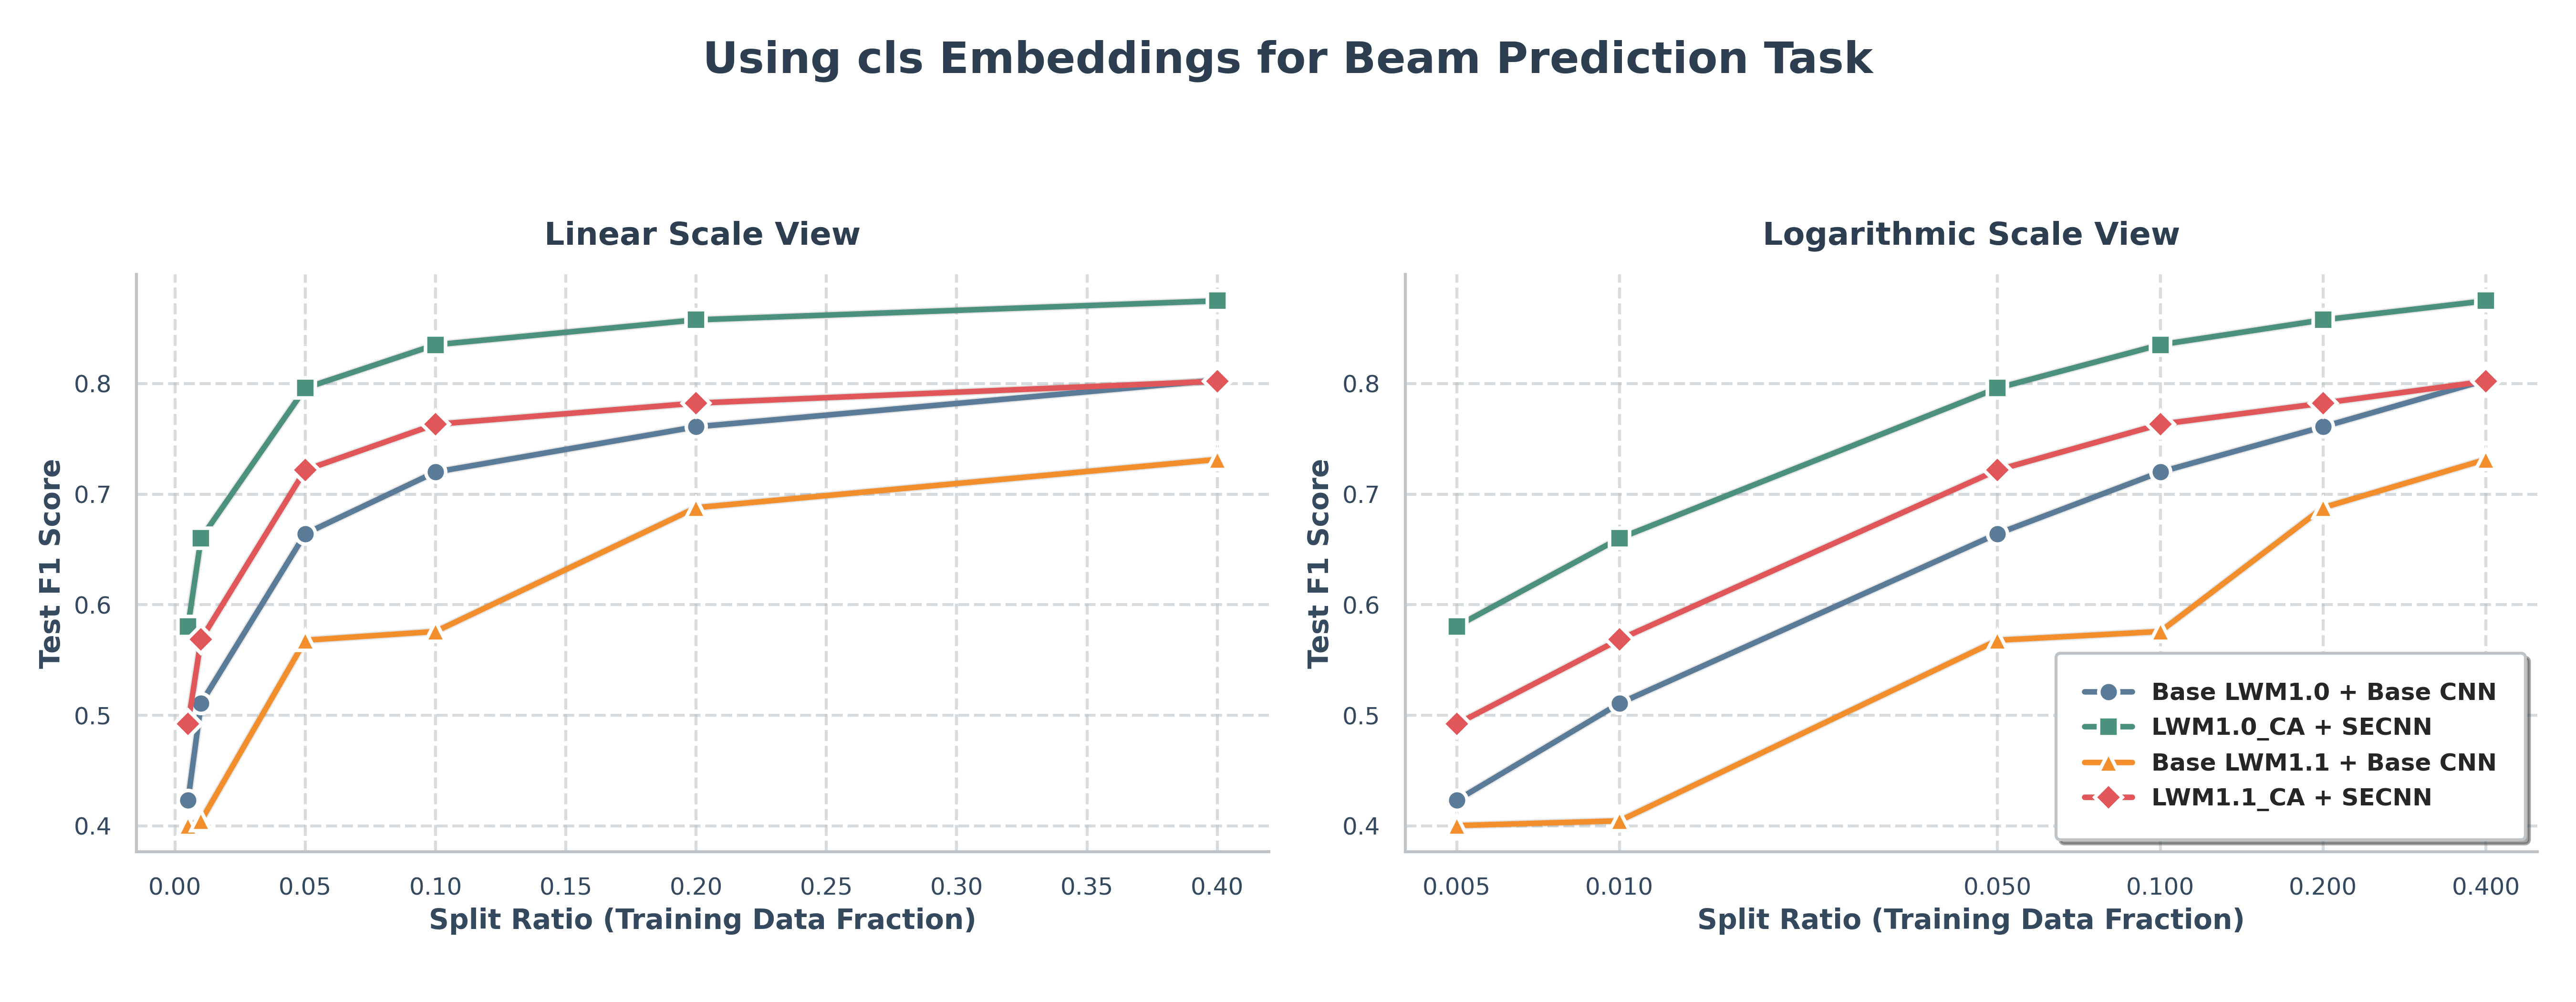
\includegraphics[width=1\textwidth]{result_photos/lwm_vs_lwm1_1_cls.png}
\end{figure}

\vspace{1.5em}
\begin{figure}[H]
\centering
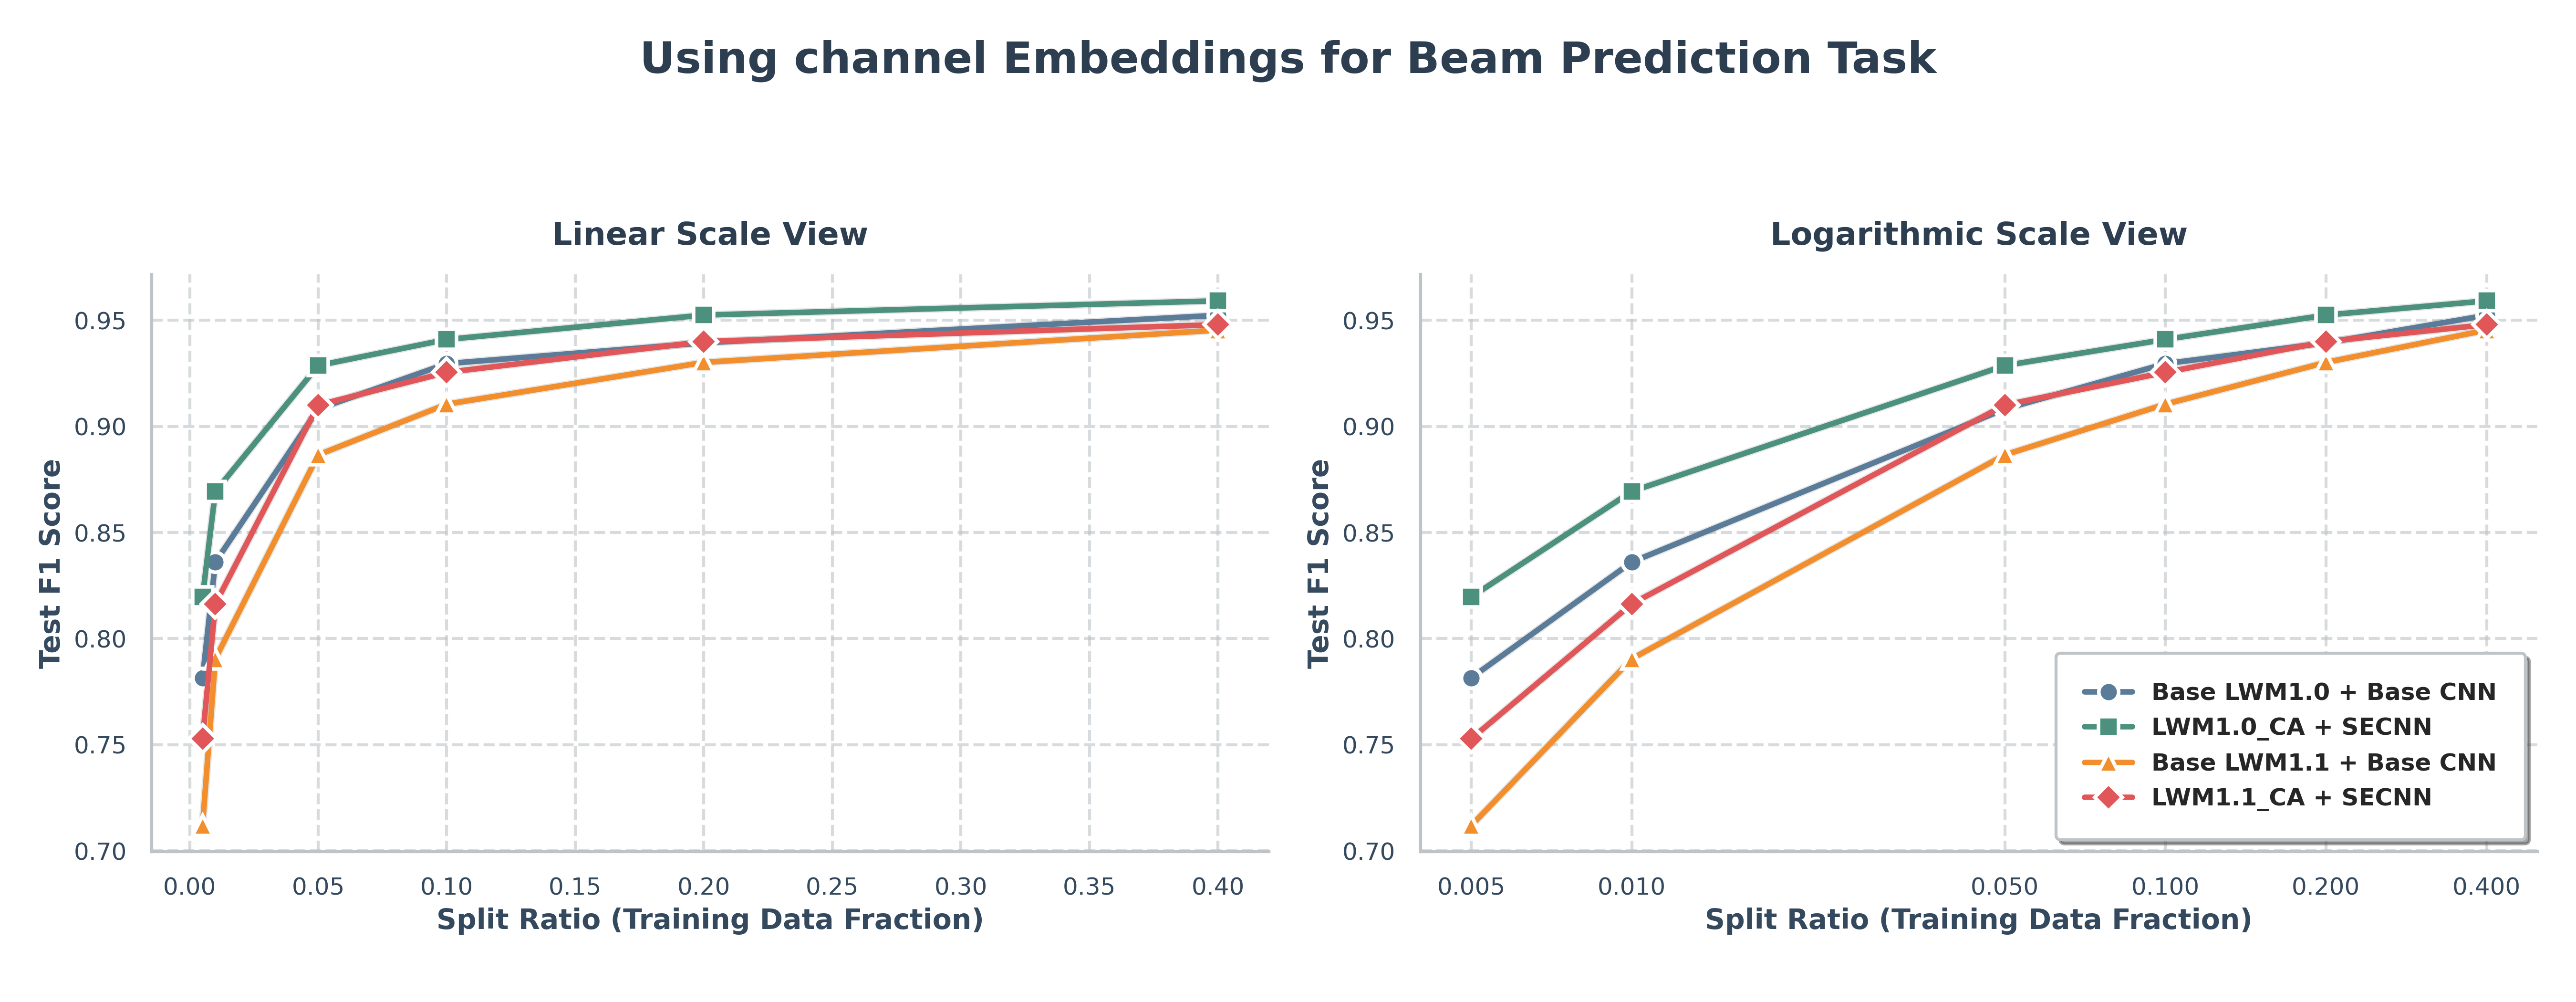
\includegraphics[width=1\textwidth]{result_photos/lwm_vs_lwm1_1_channel.png}
\caption{Generational performance comparison. Top: CLS embeddings. Bottom: Channel embeddings.}
\label{fig:results_p3}
\end{figure}

\subsection{Codebase}\label{subsec:code_p3}

\begin{itemize}[leftmargin=1.2em]
    \item \texttt{lwm1\_1/}: Vanilla LWM~1.1 backbone. \texttt{lwm\_model.py} defines the 12-layer transformer ($d{=}128$, 8 heads). \texttt{1.1\_script\_Bp\_CNN\_base.py} runs downstream beam prediction using frozen embeddings.
    \item \texttt{lwm1\_1\_ca/}: CA-augmented variant. \texttt{torch\_pipeline\_v11.py} implements the end-to-end pre-training pipeline (channel $\to$ CA $\to$ patch $\to$ mask $\to$ LWM). \texttt{coordatt.py} defines the CA block. \texttt{benchmark\_secnn.py} handles downstream evaluation. Pre-trained weights are stored as \texttt{512\_25model1\_1\_weights\_ca\_e2e.pth} (best configuration).
\end{itemize}

% ══════════════════════════════════════════════════════════════
%  6. PHASE 4: MASK-AWARE TRANSFORMER (MAT-PSEUDO)
% ══════════════════════════════════════════════════════════════
\newpage
\section{Phase 4: Mask-Aware Transformer}\label{sec:phase4}

Phases~1--3 improved the \emph{downstream head} and \emph{attention front-end} while keeping LWM's standard 12-layer transformer backbone intact. Phase~4 takes the more ambitious step of \textbf{replacing the backbone entirely} with a Mask-Aware Transformer (MAT)~\cite{mat}, aiming to match LWM's downstream accuracy at a fraction of the computational cost.

\subsection{\texorpdfstring{Architecture: MAT-Pseudo (8$\times$16)}{Architecture: MAT-Pseudo (8x16)}}\label{subsec:mat_arch}

The successful variant, \textbf{MAT-Pseudo}, preserves LWM's 128-patch tokenization while introducing mask-aware 2-D spatial attention via an $8{\times}16$ pseudo-grid reshape. The core building blocks are:

\paragraph{Window Multi-Head Attention (WindowMHA).}
Attention is computed within non-overlapping $4{\times}4$ spatial windows on the pseudo-grid. Invalid (masked) tokens receive a large negative bias ($-\tau$, $\tau{=}100$) before softmax, ensuring they are effectively ignored --- this is the \emph{mask-aware} property from~\cite{mat}. Shifted windows (cyclic roll by $w/2$) are applied in alternating stages to enable cross-window information flow.

\paragraph{Adjusted Transformer Block (ATB).}
Each ATB stage performs: WindowMHA $\to$ channel concatenation with skip $\to$ $1{\times}1$ Conv fusion $\to$ MLP (expand $3{\times}$, GELU) $\to$ $3{\times}3$ local convolution. Crucially, \textbf{no LayerNorm or BatchNorm} is used anywhere in the network. In the MAT design~\cite{mat}, normalization layers can leak spatial mask information across tokens, breaking the mask-aware inductive bias. This design choice is central to the architecture but also the root cause of the heavy variant's challenges (Section~\ref{sec:failures}).

\paragraph{Data Flow.}
\begin{enumerate}[leftmargin=1.5em]
    \item \textbf{Patching}: $(B, 2, 32, 32) \to (B, 128, 16)$ via LWM-compatible flattening.
    \item \textbf{Masking}: 15\% of patches masked (MCM-style symmetric real/imag).
    \item \textbf{Embedding}: Linear projection $16 \to 64$ + learnable positional encoding.
    \item \textbf{2-D Bridge}: $(B, 128, 64) \to (B, 64, 8, 16)$ pseudo-grid reshape.
    \item \textbf{3-stage ATB}: mask-aware attention with dynamic mask relaxation after stage~1.
    \item \textbf{Reverse Bridge}: $(B, 64, 8, 16) \to (B, 128, 64)$.
    \item \textbf{Decoder}: gather masked embeddings, project $64 \to 16$, MSE loss.
\end{enumerate}

For inference, Global Average Pooling on the pseudo-grid yields the CLS embedding $(B, 64)$, and flattening gives the channel embedding $(B, 128, 64)$ --- both LWM-compatible.

\subsection{Computational Efficiency}\label{subsec:flops}

Table~\ref{tab:flops} presents the FLOP counts and parameter budgets measured via \texttt{thop} profiling (batch size = 1). MAT-Pseudo achieves a \textbf{2.3$\times$ reduction} in FLOPs relative to LWM~1.0 while using less than half the parameters.

\begin{table}[H]
\centering
\caption{Computational cost comparison across all backbone variants.}
\label{tab:flops}
\begin{tabular}{@{}lccc@{}}
\toprule
\textbf{Model} & \textbf{FLOPs (M)} & \textbf{Parameters (K)} & \textbf{Status} \\
\midrule
LWM 1.0        & $\sim$75   & $\sim$600  & Baseline \\
LWM 1.1        & $\sim$154  & $\sim$2400 & Baseline \\
\midrule
\textbf{MAT-Pseudo (8$\times$16)}     & \textbf{33.16}  & \textbf{260}  & \checkmark \\
MAT-Pseudo + CA & 33.17  & 260  & \checkmark \\
MAT-Pseudo-Heavy & 80.35  & 630  & $\times$ (gradient explosion) \\
MAT-ViT (32$\times$32)  & 264.45 & 259  & $\times$ (lazy decoder) \\
MAT-ViT-Heavy   & 641.93 & 629  & $\times$ (failed training) \\
\bottomrule
\end{tabular}
\end{table}

\subsection{Results: MAT-Pseudo vs LWM}\label{subsec:results_p4_base}

Table~\ref{tab:mat_vs_lwm} compares MAT-Pseudo against the LWM~1.0 baselines. Both use a Base CNN downstream head.

\begin{table}[H]
\centering
\caption{MAT-Pseudo vs LWM 1.0 beam prediction F1 scores.}
\label{tab:mat_vs_lwm}
\resizebox{\textwidth}{!}{
\begin{tabular}{@{}lcccccc|cccccc@{}}
\toprule
 & \multicolumn{6}{c}{\textbf{CLS Embedding}} & \multicolumn{6}{c}{\textbf{Channel Embedding}} \\
\cmidrule(lr){2-7} \cmidrule(l){8-13}
\textbf{Ratio ($r$)} & \textbf{0.5\%} & \textbf{1\%} & \textbf{5\%} & \textbf{10\%} & \textbf{20\%} & \textbf{40\%} & \textbf{0.5\%} & \textbf{1\%} & \textbf{5\%} & \textbf{10\%} & \textbf{20\%} & \textbf{40\%} \\
\midrule
Base LWM 1.0 + Base CNN & 0.4231 & 0.5108 & 0.6642 & 0.7200 & 0.7609 & 0.8031 & 0.7815 & 0.8361 & 0.9082 & 0.9296 & 0.9394 & 0.9524 \\
MAT-Pseudo + Base CNN    & \textbf{0.4598} & \textbf{0.5761} & \textbf{0.6821} & \textbf{0.7720} & \textbf{0.7983} & \textbf{0.8188} & 0.7327 & 0.8209 & \textbf{0.9089} & 0.9244 & 0.9380 & 0.9466 \\
\bottomrule
\end{tabular}}
\end{table}

\begin{figure}[H]
\centering
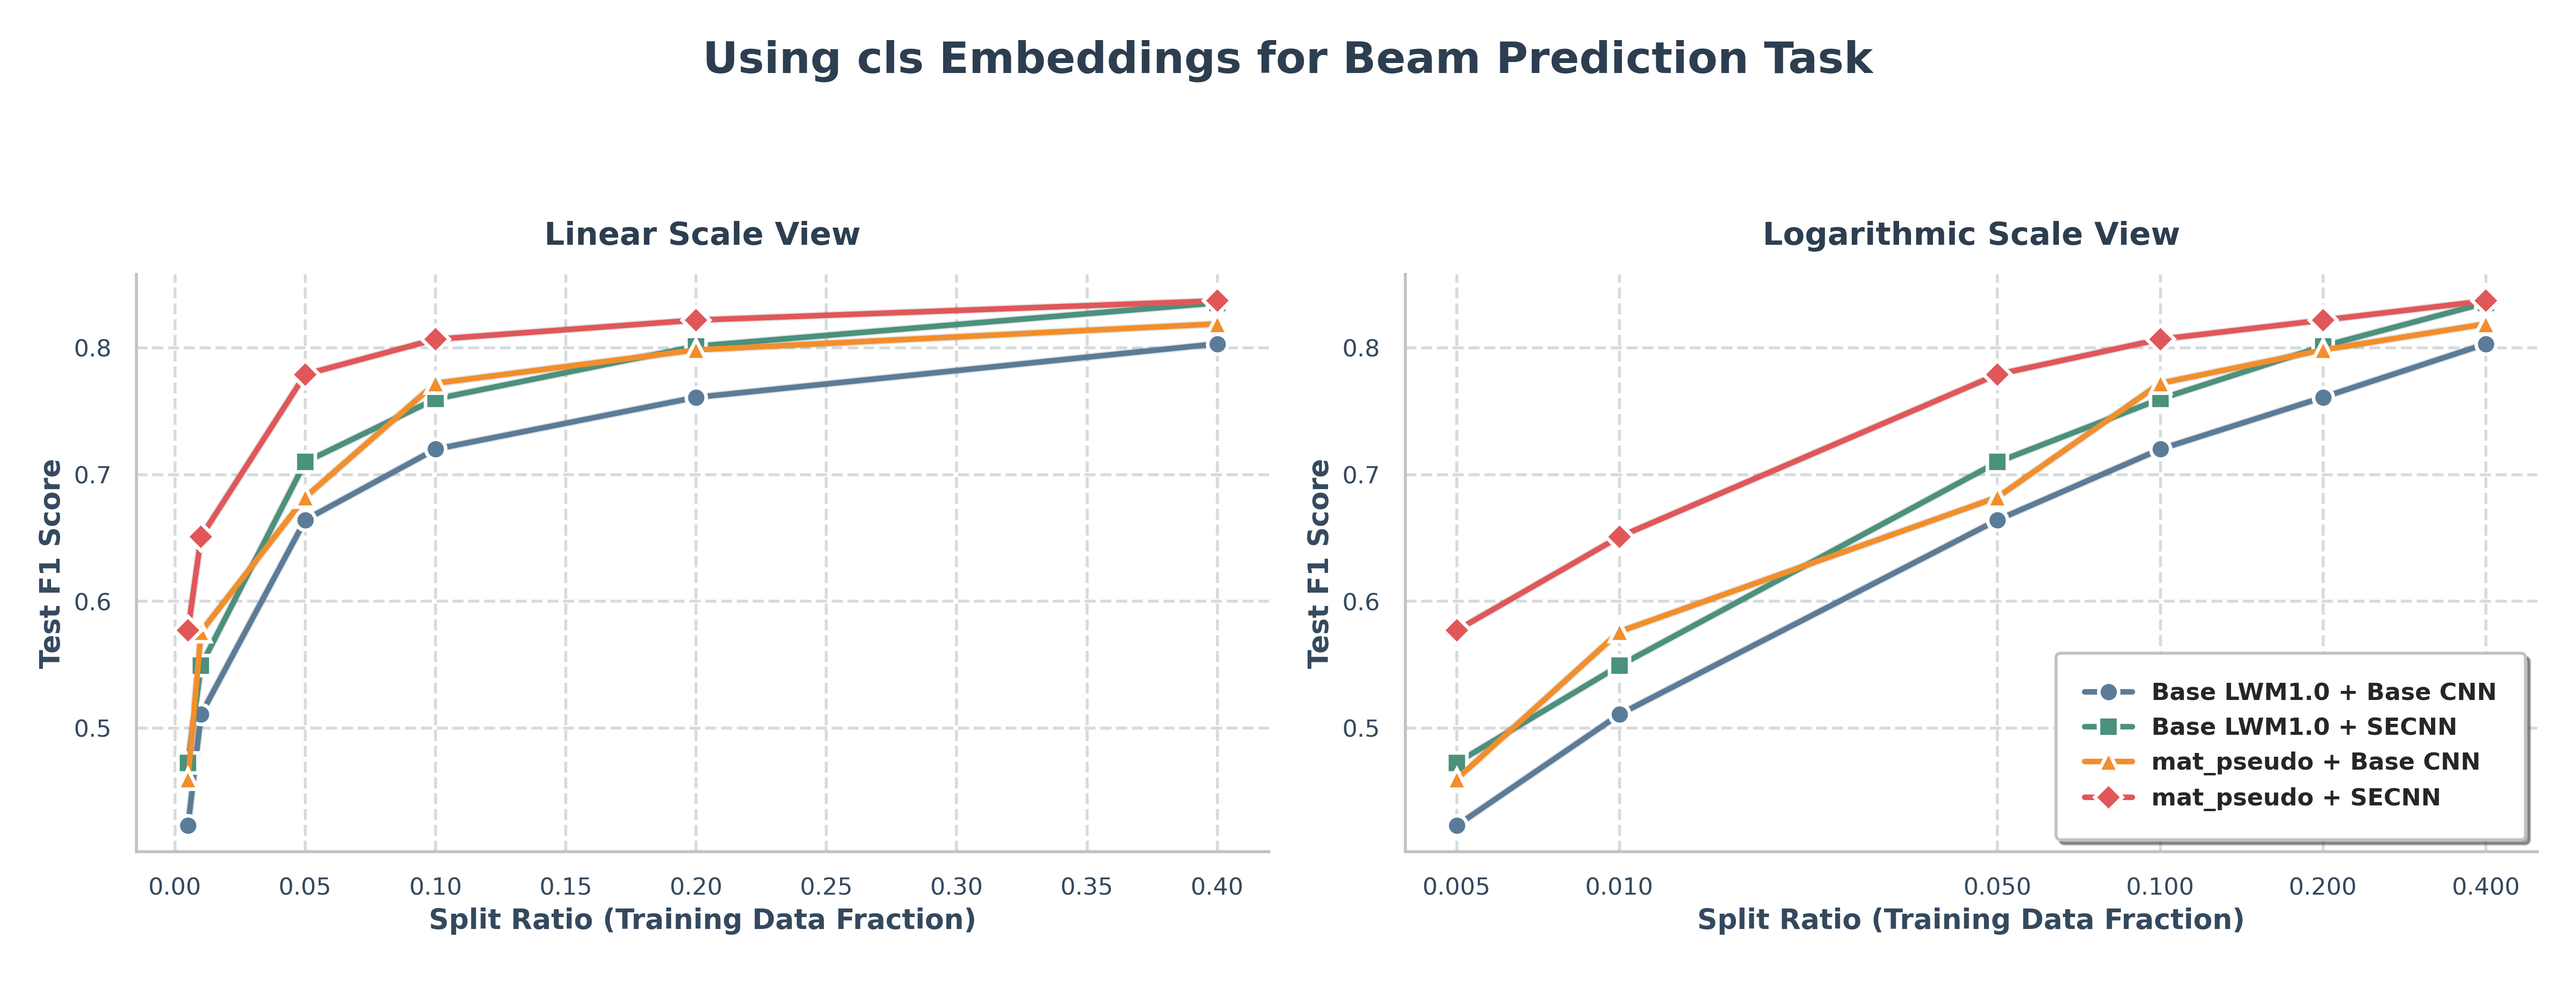
\includegraphics[width=1\textwidth]{result_photos/mat_pseudo_vs_lwm_cls.png}
\end{figure}

\vspace{1.5em}
\begin{figure}[H]
\centering
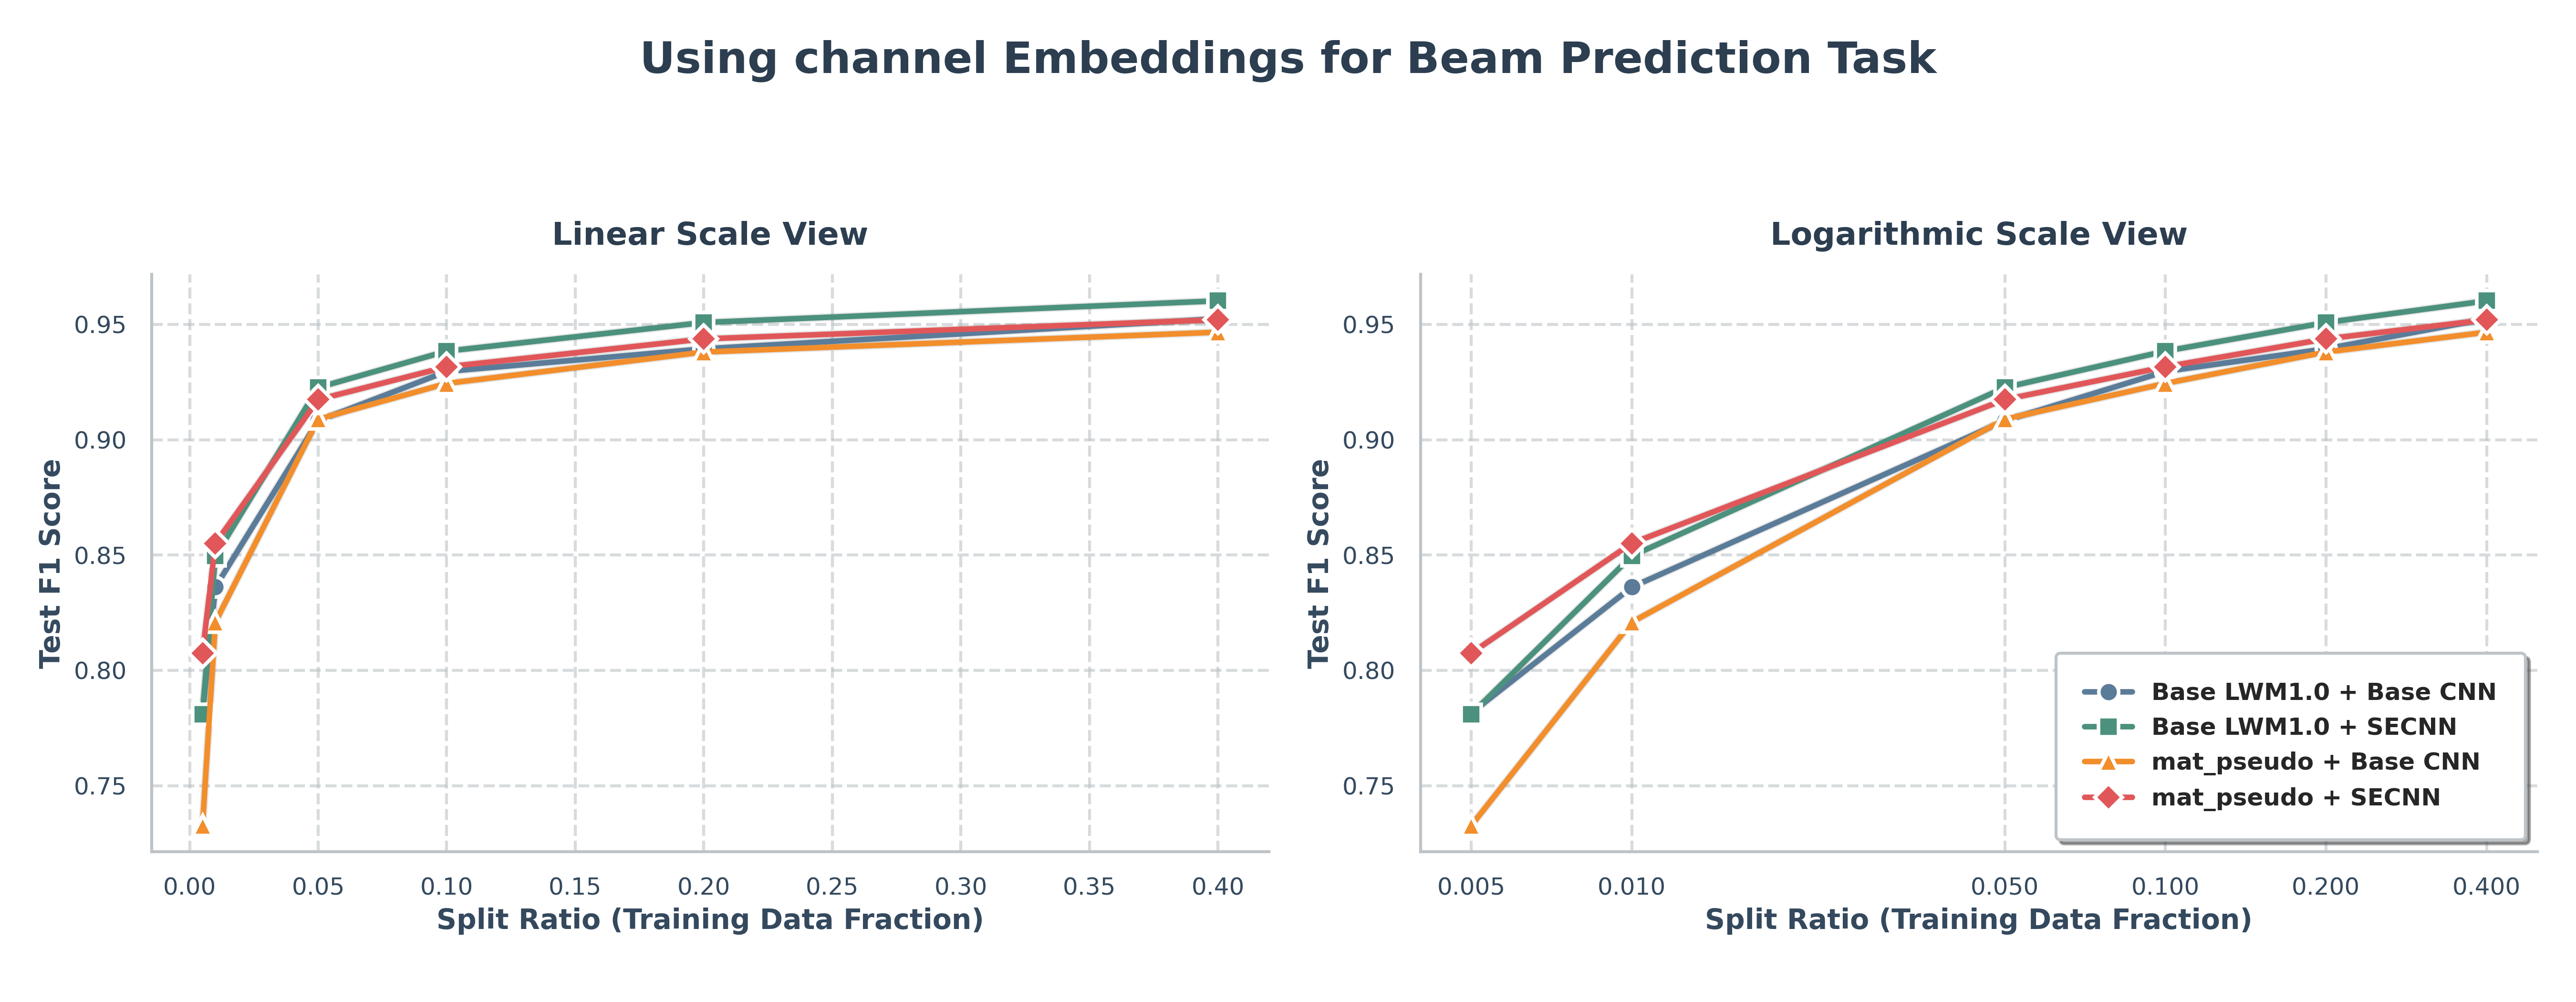
\includegraphics[width=1\textwidth]{result_photos/mat_pseudo_vs_lwm_channel.png}
\caption{MAT-Pseudo vs LWM 1.0 (Base CNN head). Top: CLS. Bottom: Channel.}
\label{fig:mat_vs_lwm}
\end{figure}

\paragraph{Inferences.}
\begin{enumerate}
    \item \textbf{CLS parity at 2.3$\times$ less compute.} MAT-Pseudo matches or exceeds LWM~1.0 on CLS embeddings across all split ratios (+3.7\,pp at $r{=}0.005$, +6.5\,pp at $r{=}0.01$, +5.2\,pp at $r{=}0.1$), despite using only 33M FLOPs vs LWM's 75M.

    \item \textbf{Channel embedding trade-off.} At the lowest split ratio ($r{=}0.005$), MAT-Pseudo trails LWM by $-$4.9\,pp on channel embeddings. This gap closes rapidly: by $r{=}0.05$ the models are within 0.1\,pp. The initial deficit is attributable to the smaller model capacity (260K vs 600K parameters) being insufficient to fully resolve the 128$\times$64 channel manifold with minimal supervision.

    \item \textbf{Efficiency frontier.} MAT-Pseudo establishes a new efficiency frontier: it is the only model in our evaluation that achieves LWM-competitive accuracy with sub-35M FLOPs, making it viable for edge deployment in latency-sensitive wireless systems.
\end{enumerate}

\subsection{CA Integration: MAT-Pseudo-CA}\label{subsec:mat_ca}

Following the established pattern from Phases~2 and~3, Coordinate Attention (Section~\ref{subsec:ca}, Figure~\ref{fig:coord_att}) is integrated as a front-end to MAT-Pseudo. The CA module recalibrates the raw $(B, 2, 32, 32)$ channel before patching, adding only 76 parameters and negligible FLOPs ($<$0.01M). Table~\ref{tab:mat_ca_vs_lwm_ca} compares the CA-augmented variants.

\begin{table}[H]
\centering
\caption{MAT-Pseudo-CA vs LWM-CA beam prediction F1 scores (SECNN head).}
\label{tab:mat_ca_vs_lwm_ca}
\resizebox{\textwidth}{!}{
\begin{tabular}{@{}lcccccc|cccccc@{}}
\toprule
 & \multicolumn{6}{c}{\textbf{CLS Embedding}} & \multicolumn{6}{c}{\textbf{Channel Embedding}} \\
\cmidrule(lr){2-7} \cmidrule(l){8-13}
\textbf{Ratio ($r$)} & \textbf{0.5\%} & \textbf{1\%} & \textbf{5\%} & \textbf{10\%} & \textbf{20\%} & \textbf{40\%} & \textbf{0.5\%} & \textbf{1\%} & \textbf{5\%} & \textbf{10\%} & \textbf{20\%} & \textbf{40\%} \\
\midrule
LWM 1.0\_CA + SECNN       & 0.5805 & 0.6601 & 0.7959 & 0.8351 & 0.8576 & 0.8748 & 0.8196 & 0.8694 & 0.9287 & 0.9410 & 0.9525 & 0.9592 \\
MAT-Pseudo-CA + SECNN & \textbf{0.6219} & \textbf{0.6821} & 0.7917 & 0.8202 & 0.8390 & 0.8515 & 0.8139 & 0.8641 & 0.9213 & 0.9354 & 0.9452 & 0.9536 \\
\bottomrule
\end{tabular}}
\end{table}

\begin{figure}[H]
\centering
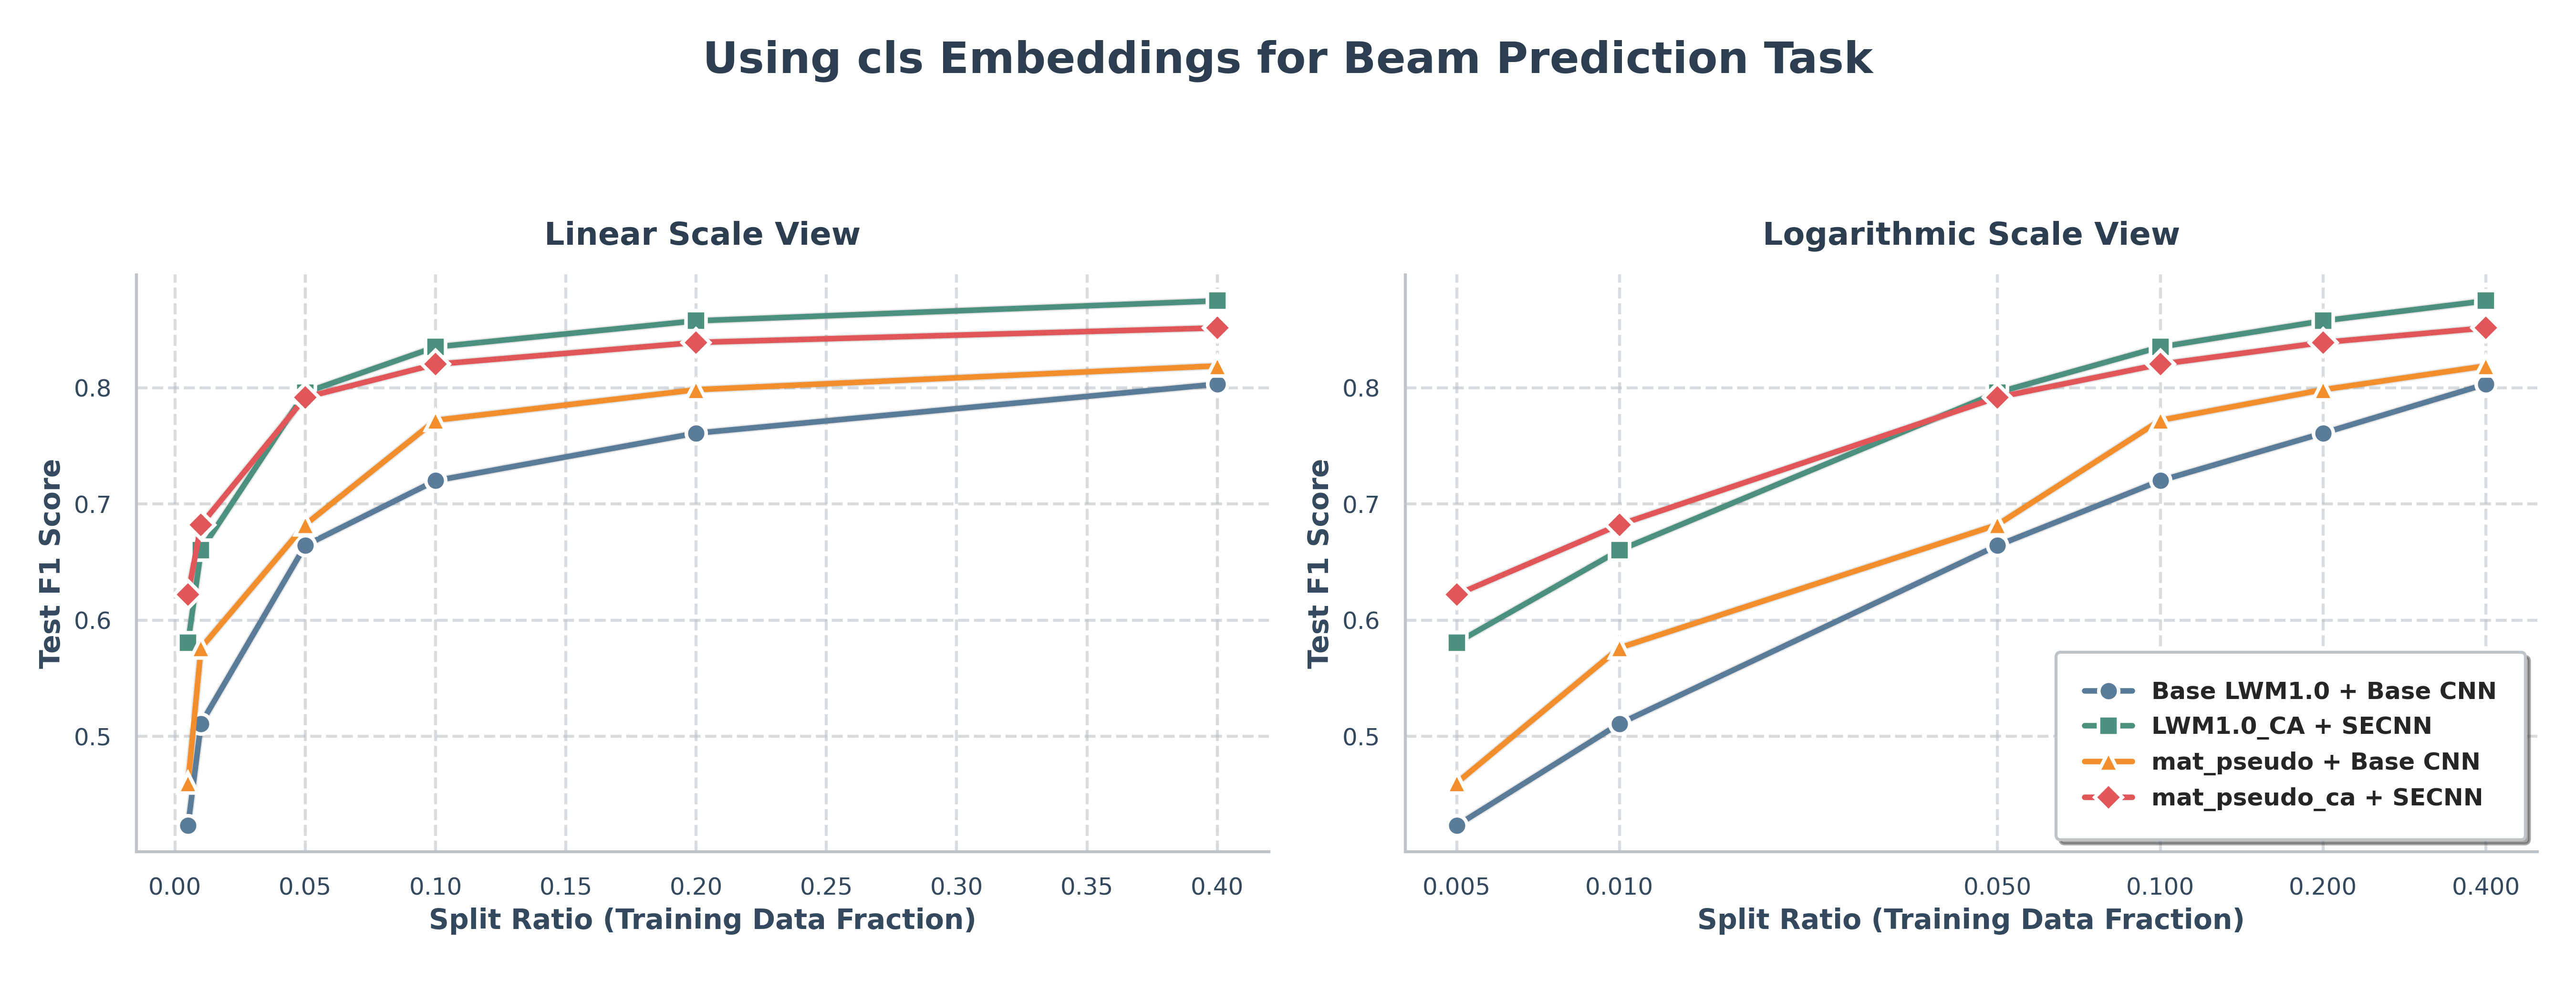
\includegraphics[width=1\textwidth]{result_photos/mat_pseudo_ca_vs_lwm_ca_cls.png}
\end{figure}

\vspace{1.5em}
\begin{figure}[H]
\centering
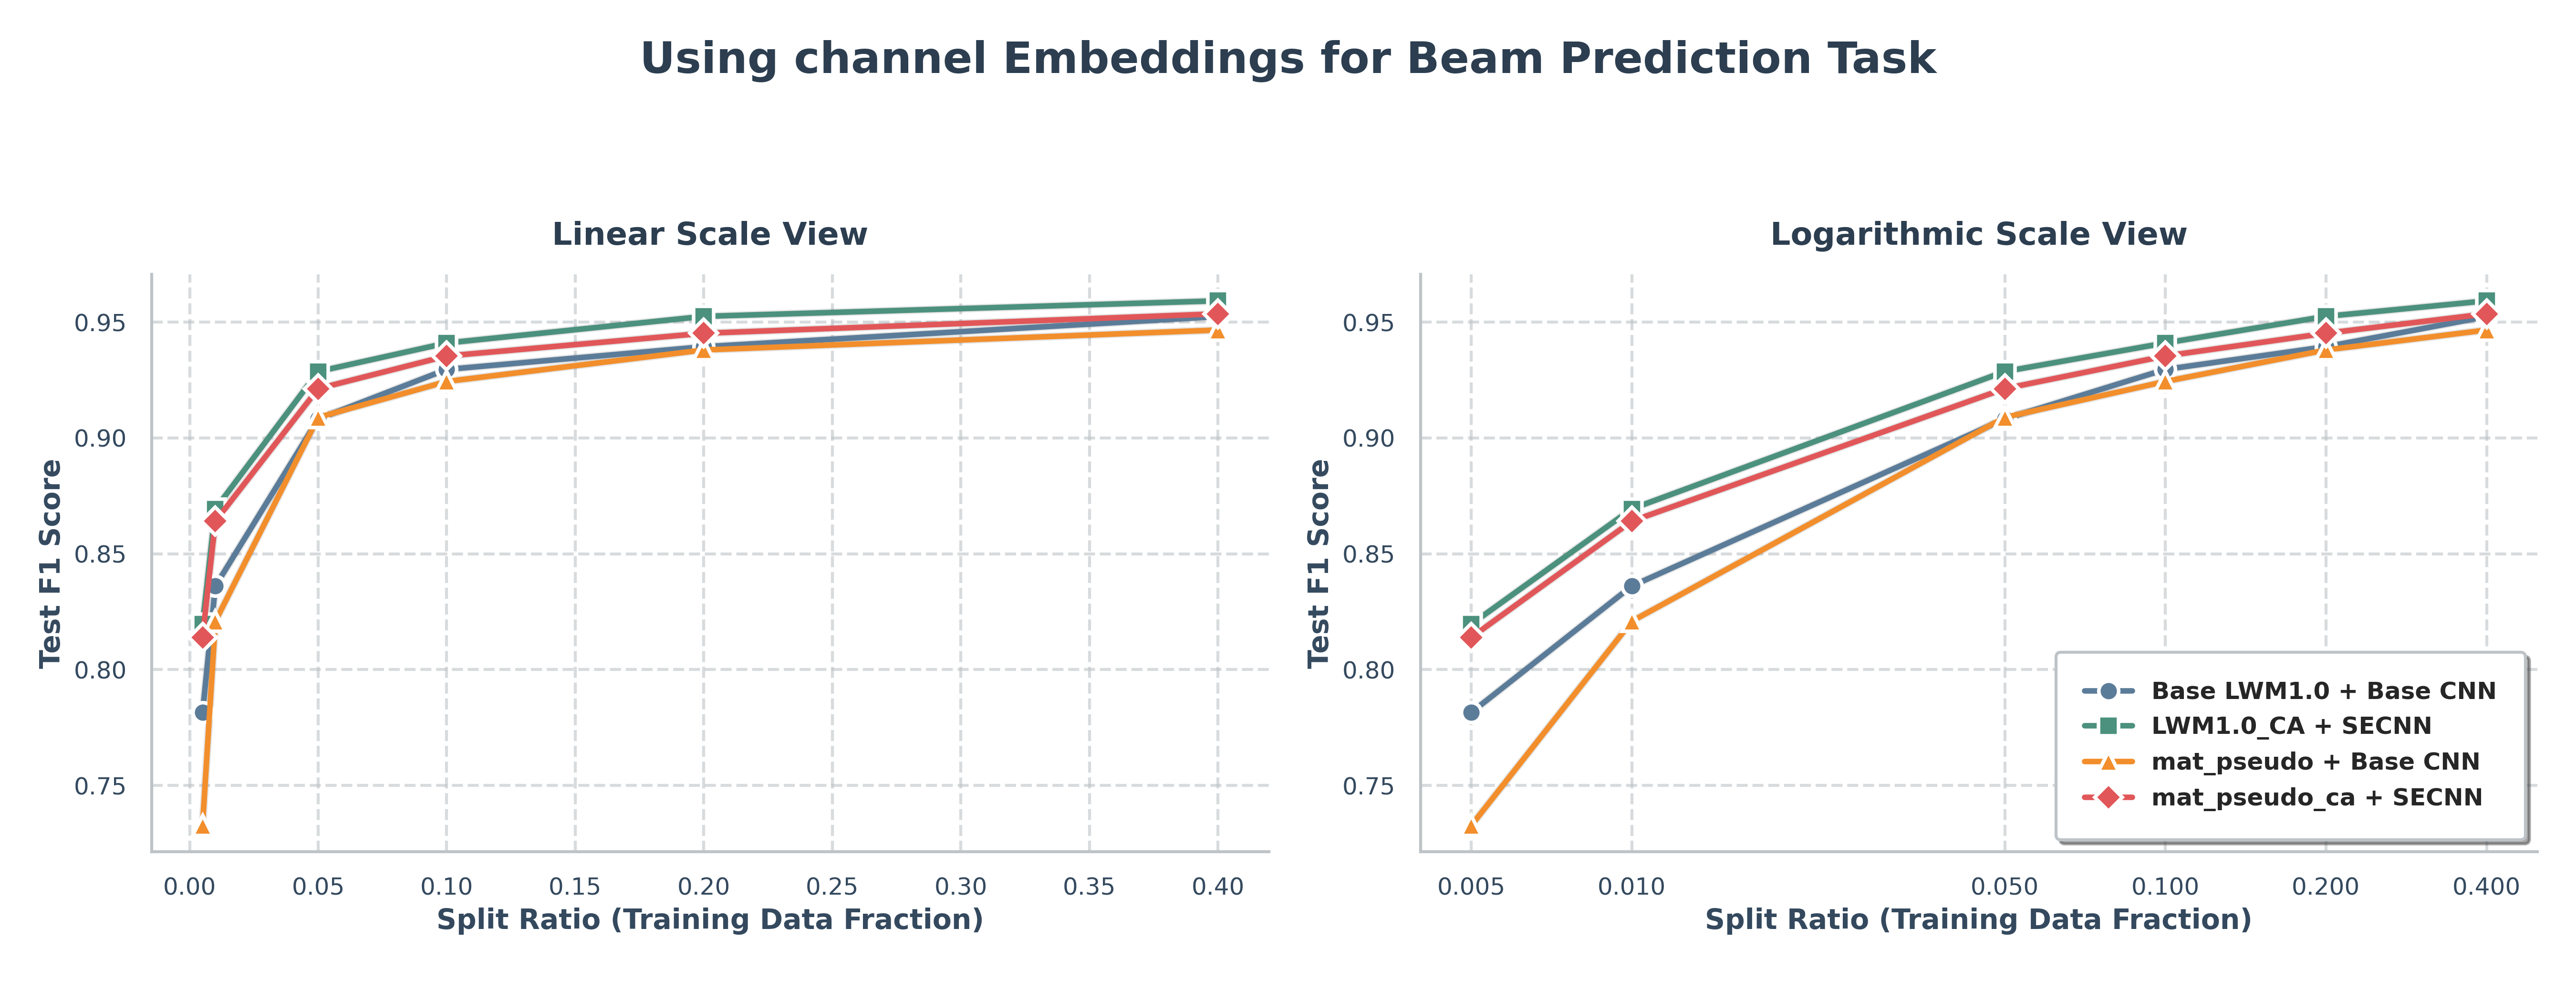
\includegraphics[width=1\textwidth]{result_photos/mat_pseudo_ca_vs_lwm_ca_channel.png}
\caption{MAT-Pseudo-CA vs LWM-CA (SECNN head). Top: CLS. Bottom: Channel.}
\label{fig:mat_ca_vs_lwm_ca}
\end{figure}

\paragraph{Inferences.}
\begin{enumerate}
    \item \textbf{Low-data superiority.} MAT-Pseudo-CA outperforms LWM-CA on CLS embeddings at the critical low-data points: +4.1\,pp at $r{=}0.005$ and +2.2\,pp at $r{=}0.01$. This is remarkable given that MAT-Pseudo operates at \textbf{less than half} the FLOPs of LWM~1.0.

    \item \textbf{Convergence gap at high data.} At $r \ge 0.05$, LWM-CA retakes the lead by 0.4--2.3\,pp. The larger capacity of LWM (600K vs 260K params) allows it to absorb more supervision. This suggests that a moderately scaled MAT variant (e.g., $d{=}96$) could close this gap while remaining well below LWM's FLOP budget.

    \item \textbf{Channel embedding near-parity.} On channel embeddings, both models are within $\sim$0.6\,pp across all splits, confirming that the 128$\times$64 spatial embedding is rich enough to saturate the SECNN head regardless of the backbone's total capacity.
\end{enumerate}

\paragraph{Effect of CA on Pre-training Convergence.}
Figure~\ref{fig:mat_ca_progress} shows the pre-training loss curves for MAT-Pseudo with and without Coordinate Attention. The CA variant converges faster and to a lower final loss, demonstrating that the spatial priors injected by CA improve not only downstream performance but also the quality of the self-supervised pre-training itself.

\begin{figure}[H]
\centering

\includegraphics[width=0.85\textwidth]{exp_photos/mat_pseudo_compare_progress.png}
\caption{Pre-training loss comparison: MAT-Pseudo vs MAT-Pseudo-CA. The CA front-end accelerates convergence and reduces the final MCM loss.}
\label{fig:mat_ca_progress}
\end{figure}

\subsection{Codebase}\label{subsec:code_p4}

\begin{itemize}[leftmargin=1.2em]
    \item \texttt{mask\_aware\_tf/}: Core MAT implementations. \texttt{mat\_vit\_lwm.py} defines \texttt{WindowMHA} and \texttt{ATB}. \texttt{mat\_pseudo\_lwm.py} implements the MAT-Pseudo model. \texttt{pretrain\_pseudo.py} handles MCM pre-training. \texttt{mat\_script\_DownstreamBp.py} runs downstream evaluation. Weights: \texttt{512\_100mat\_pseudo\_lwm\_weights.pth}.

    \item \texttt{mat\_pseudo\_lwm\_ca/}: CA-augmented MAT-Pseudo. \texttt{mat\_pseudo\_lwm\_ca.py} extends MAT-Pseudo with a CoordAtt front-end. \texttt{pretrain\_pseudo\_ca.py} handles joint pre-training. \texttt{mat\_ca\_script\_DownstreamBp.py} evaluates beam prediction. Weights: \texttt{512\_100mat\_pseudo\_lwm\_ca\_weights.pth}.

    \item \texttt{mask\_aware\_tf\_heavy/}: Scaled variants (MAT-Pseudo-Heavy, MAT-ViT-Heavy) used in the experimental exploration (Section~\ref{sec:failures}).
\end{itemize}

All downstream scripts extract frozen embeddings from the pre-trained MAT backbone and train only the CNN head.

% ══════════════════════════════════════════════════════════════
%  7. ARCHITECTURAL EXPLORATION AND INSIGHTS
% ══════════════════════════════════════════════════════════════
\newpage
\section{Architectural Exploration and Insights}\label{sec:failures}

During the development of the MAT backbone, four architectural variants were explored. Only MAT-Pseudo converged to useful representations. This section documents the remaining three variants and the design insights gained from each experiment.

\subsection{MAT-Pseudo-Heavy}\label{subsec:fail_heavy}

\textbf{Goal:} Scale MAT-Pseudo to match LWM's depth (80M FLOPs, 630K parameters) for potentially higher accuracy.

\textbf{Architecture:} Identical to MAT-Pseudo but with increased $d_\text{model}$ and additional ATB stages, roughly tripling the parameter count and FLOPs.

\textbf{Failure mode: Catastrophic gradient explosion.} The removal of all normalization layers (LayerNorm, BatchNorm) --- necessary to prevent spatial mask leakage in the MAT architecture --- left the deeper network without any mechanism to bound activation magnitudes. While the 3-stage MAT-Pseudo (260K params) can sustain stable gradients, the heavier variant rapidly diverges during pre-training, with loss values growing unbounded within the first few epochs. An attempt to mitigate this with \texttt{DynamicTanh} (a learnable per-channel $\tanh$ normalization) was also unsuccessful.

\textbf{Downstream results} confirm total failure: F1 scores plateau at $\sim$0.35--0.43 across all split ratios (Table~\ref{tab:flops}), indicating that the encoder learned no meaningful representations.

\begin{figure}[H]
\centering

\includegraphics[width=0.85\textwidth]{exp_photos/mat_ExPlOdEd_pseudo_heavy_progress.png}
\caption{MAT-Pseudo-Heavy training loss. The loss diverges catastrophically due to the absence of normalization layers in the scaled architecture.}
\label{fig:heavy_fail}
\end{figure}

\subsection{\texorpdfstring{MAT-ViT (32$\times$32)}{MAT-ViT (32x32)}}\label{subsec:fail_vit}

\textbf{Goal:} Operate directly on the full $32{\times}32$ spatial grid (instead of the $8{\times}16$ pseudo-grid), potentially capturing finer spatial structure.

\textbf{Architecture:} Input $(B, 2, 32, 32) \to 1{\times}1$ Conv $\to (B, 64, 32, 32) \to$ spatial masking $\to$ 3-stage ATB $\to 1{\times}1$ Conv decoder $\to (B, 2, 32, 32)$. CLS embedding via GAP; channel embedding via \texttt{AdaptiveAvgPool2d(8,16)}.

\textbf{Failure mode: Lazy decoder / encoder collapse.} The pre-training loss converged to a low value ($\sim$0.3), suggesting the model was learning. However, downstream F1 scores were poor and erratic (e.g., channel embedding F1 dropping from 0.64 at $r{=}0.005$ to 0.42 at $r{=}0.01$, then recovering at higher splits). This non-monotonic behavior indicates that the \emph{decoder} memorized reconstruction patterns while the \emph{encoder} failed to extract robust, transferable features. A likely contributing factor is the absence of 2-D positional encodings: without explicit spatial priors, the $32{\times}32$ grid is too large for the 3-stage ATB to establish meaningful long-range dependencies.

\begin{figure}[H]
\centering

\includegraphics[width=0.85\textwidth]{exp_photos/mat_vit_progress.png}
\caption{MAT-ViT pre-training loss. The loss converges smoothly, masking the underlying encoder collapse that is only revealed during downstream evaluation.}
\label{fig:vit_fail}
\end{figure}

\subsection{\texorpdfstring{MAT-ViT-Heavy (32$\times$32)}{MAT-ViT-Heavy (32x32)}}\label{subsec:fail_vit_heavy}

\textbf{Goal:} Scale MAT-ViT to 642M FLOPs / 629K parameters.

\textbf{Failure:} Combined both failure modes --- the gradient instability from the normalization-free deep architecture and the lazy decoder problem from the $32{\times}32$ grid. Training was abandoned early.

\subsection{Key Takeaways}\label{subsec:fail_lessons}

\begin{enumerate}
    \item \textbf{Normalization is critical for depth scaling.} The MAT constraint of no LN/BN fundamentally limits the viable model depth. Future work could explore alternatives such as \texttt{RMSNorm} (which operates per-token rather than spatially) or gradient clipping strategies.

    \item \textbf{Pseudo-grid is the right abstraction.} The $8{\times}16$ pseudo-grid strikes the optimal balance between spatial resolution and the ATB's receptive field. The $32{\times}32$ grid is too large for $4{\times}4$ windows, leading to encoder collapse.

    \item \textbf{Low pre-training loss $\neq$ good embeddings.} MAT-ViT's smooth convergence demonstrates that reconstruction loss alone is an insufficient proxy for downstream quality --- the decoder can memorize without the encoder learning transferable features.
\end{enumerate}

% ══════════════════════════════════════════════════════════════
%  REFERENCES
% ══════════════════════════════════════════════════════════════
\newpage
\begin{thebibliography}{9}

\bibitem{lwm}
S.~Alikhani, G.~Charan, and A.~Alkhateeb,
``Large Wireless Model (LWM): A Foundation Model for Wireless Channels,''
\textit{arXiv preprint arXiv:2411.08872v1}, Nov.~2024.

\bibitem{lwm11}
S.~Alikhani, G.~Charan, and A.~Alkhateeb,
``Large Wireless Model (LWM): A Foundation Model for Wireless Channels,''
\textit{arXiv preprint arXiv:2411.08872v2}, Apr.~2025.

\bibitem{mat}
W.~Li, Z.~Lin, K.~Zhou, L.~Qi, Y.~Wang, and J.~Jia,
``MAT: Mask-Aware Transformer for Large Hole Image Inpainting,''
in \textit{Proc.\ IEEE/CVF Conference on Computer Vision and Pattern Recognition (CVPR)}, pp.~10758--10768, 2022.

\end{thebibliography}

\end{document}
